\documentclass[1p]{elsarticle_modified}
%\bibliographystyle{elsarticle-num}

%\usepackage[colorlinks]{hyperref}
%\usepackage{abbrmath_seonhwa} %\Abb, \Ascr, \Acal ,\Abf, \Afrak
\usepackage{amsfonts}
\usepackage{amssymb}
\usepackage{amsmath}
\usepackage{amsthm}
\usepackage{scalefnt}
\usepackage{amsbsy}
\usepackage{kotex}
\usepackage{caption}
\usepackage{subfig}
\usepackage{color}
\usepackage{graphicx}
\usepackage{xcolor} %% white, black, red, green, blue, cyan, magenta, yellow
\usepackage{float}
\usepackage{setspace}
\usepackage{hyperref}

\usepackage{tikz}
\usetikzlibrary{arrows}

\usepackage{multirow}
\usepackage{array} % fixed length table
\usepackage{hhline}

%%%%%%%%%%%%%%%%%%%%%
\makeatletter
\renewcommand*\env@matrix[1][\arraystretch]{%
	\edef\arraystretch{#1}%
	\hskip -\arraycolsep
	\let\@ifnextchar\new@ifnextchar
	\array{*\c@MaxMatrixCols c}}
\makeatother %https://tex.stackexchange.com/questions/14071/how-can-i-increase-the-line-spacing-in-a-matrix
%%%%%%%%%%%%%%%

\usepackage[normalem]{ulem}

\newcommand{\msout}[1]{\ifmmode\text{\sout{\ensuremath{#1}}}\else\sout{#1}\fi}
%SOURCE: \msout is \stkout macro in https://tex.stackexchange.com/questions/20609/strikeout-in-math-mode

\newcommand{\cancel}[1]{
	\ifmmode
	{\color{red}\msout{#1}}
	\else
	{\color{red}\sout{#1}}
	\fi
}

\newcommand{\add}[1]{
	{\color{blue}\uwave{#1}}
}

\newcommand{\replace}[2]{
	\ifmmode
	{\color{red}\msout{#1}}{\color{blue}\uwave{#2}}
	\else
	{\color{red}\sout{#1}}{\color{blue}\uwave{#2}}
	\fi
}

\newcommand{\Sol}{\mathcal{S}} %segment
\newcommand{\D}{D} %diagram
\newcommand{\A}{\mathcal{A}} %arc


%%%%%%%%%%%%%%%%%%%%%%%%%%%%%5 test

\def\sl{\operatorname{\textup{SL}}(2,\Cbb)}
\def\psl{\operatorname{\textup{PSL}}(2,\Cbb)}
\def\quan{\mkern 1mu \triangleright \mkern 1mu}

\theoremstyle{definition}
\newtheorem{thm}{Theorem}[section]
\newtheorem{prop}[thm]{Proposition}
\newtheorem{lem}[thm]{Lemma}
\newtheorem{ques}[thm]{Question}
\newtheorem{cor}[thm]{Corollary}
\newtheorem{defn}[thm]{Definition}
\newtheorem{exam}[thm]{Example}
\newtheorem{rmk}[thm]{Remark}
\newtheorem{alg}[thm]{Algorithm}

\newcommand{\I}{\sqrt{-1}}
\begin{document}

%\begin{frontmatter}
%
%\title{Boundary parabolic representations of knots up to 8 crossings}
%
%%% Group authors per affiliation:
%\author{Yunhi Cho} 
%\address{Department of Mathematics, University of Seoul, Seoul, Korea}
%\ead{yhcho@uos.ac.kr}
%
%
%\author{Seonhwa Kim} %\fnref{s_kim}}
%\address{Center for Geometry and Physics, Institute for Basic Science, Pohang, 37673, Korea}
%\ead{ryeona17@ibs.re.kr}
%
%\author{Hyuk Kim}
%\address{Department of Mathematical Sciences, Seoul National University, Seoul 08826, Korea}
%\ead{hyukkim@snu.ac.kr}
%
%\author{Seokbeom Yoon}
%\address{Department of Mathematical Sciences, Seoul National University, Seoul, 08826,  Korea}
%\ead{sbyoon15@snu.ac.kr}
%
%\begin{abstract}
%We find all boundary parabolic representation of knots up to 8 crossings.
%
%\end{abstract}
%\begin{keyword}
%    \MSC[2010] 57M25 
%\end{keyword}
%
%\end{frontmatter}

%\linenumbers
%\tableofcontents
%
\newcommand\colored[1]{\textcolor{white}{\rule[-0.35ex]{0.8em}{1.4ex}}\kern-0.8em\color{red} #1}%
%\newcommand\colored[1]{\textcolor{white}{ #1}\kern-2.17ex	\textcolor{white}{ #1}\kern-1.81ex	\textcolor{white}{ #1}\kern-2.15ex\color{red}#1	}

{\Large $\underline{12a_{1195}~(K12a_{1195})}$}

\setlength{\tabcolsep}{10pt}
\renewcommand{\arraystretch}{1.6}
\vspace{1cm}\begin{tabular}{m{100pt}>{\centering\arraybackslash}m{274pt}}
\multirow{5}{120pt}{
	\centering
	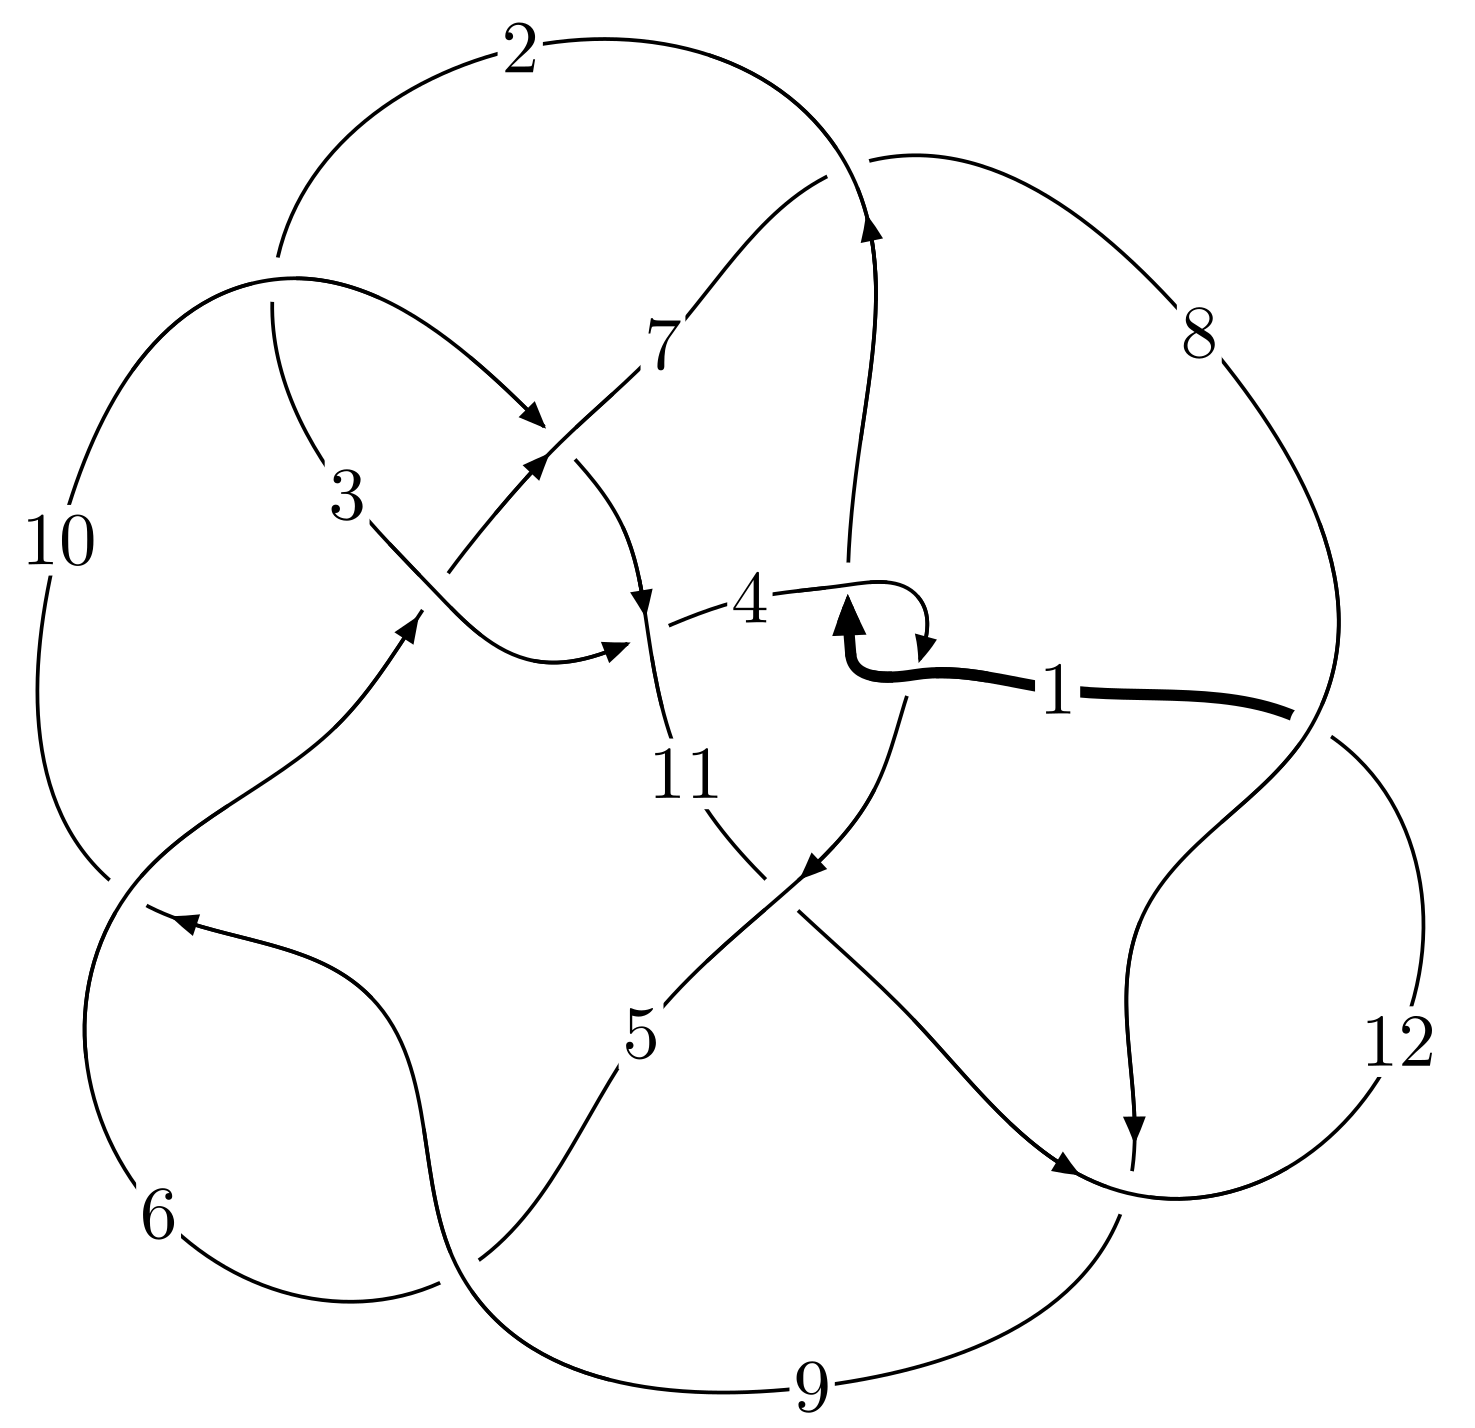
\includegraphics[width=112pt]{../../../GIT/diagram.site/Diagrams/png/1996_12a_1195.png}\\
\ \ \ A knot diagram\footnotemark}&
\allowdisplaybreaks
\textbf{Linearized knot diagam} \\
\cline{2-2}
 &
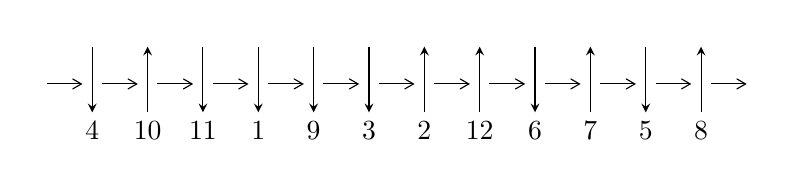
\begin{tikzpicture}[x=20pt, y=17pt]
	% nodes
	\node (C0) at (0, 0) {};
	\node (C1) at (1, 0) {};
	\node (C1U) at (1, +1) {};
	\node (C1D) at (1, -1) {4};

	\node (C2) at (2, 0) {};
	\node (C2U) at (2, +1) {};
	\node (C2D) at (2, -1) {10};

	\node (C3) at (3, 0) {};
	\node (C3U) at (3, +1) {};
	\node (C3D) at (3, -1) {11};

	\node (C4) at (4, 0) {};
	\node (C4U) at (4, +1) {};
	\node (C4D) at (4, -1) {1};

	\node (C5) at (5, 0) {};
	\node (C5U) at (5, +1) {};
	\node (C5D) at (5, -1) {9};

	\node (C6) at (6, 0) {};
	\node (C6U) at (6, +1) {};
	\node (C6D) at (6, -1) {3};

	\node (C7) at (7, 0) {};
	\node (C7U) at (7, +1) {};
	\node (C7D) at (7, -1) {2};

	\node (C8) at (8, 0) {};
	\node (C8U) at (8, +1) {};
	\node (C8D) at (8, -1) {12};

	\node (C9) at (9, 0) {};
	\node (C9U) at (9, +1) {};
	\node (C9D) at (9, -1) {6};

	\node (C10) at (10, 0) {};
	\node (C10U) at (10, +1) {};
	\node (C10D) at (10, -1) {7};

	\node (C11) at (11, 0) {};
	\node (C11U) at (11, +1) {};
	\node (C11D) at (11, -1) {5};

	\node (C12) at (12, 0) {};
	\node (C12U) at (12, +1) {};
	\node (C12D) at (12, -1) {8};
	\node (C13) at (13, 0) {};

	% arrows
	\draw[->,>={angle 60}]
	(C0) edge (C1) (C1) edge (C2) (C2) edge (C3) (C3) edge (C4) (C4) edge (C5) (C5) edge (C6) (C6) edge (C7) (C7) edge (C8) (C8) edge (C9) (C9) edge (C10) (C10) edge (C11) (C11) edge (C12) (C12) edge (C13) ;	\draw[->,>=stealth]
	(C1U) edge (C1D) (C2D) edge (C2U) (C3U) edge (C3D) (C4U) edge (C4D) (C5U) edge (C5D) (C6U) edge (C6D) (C7D) edge (C7U) (C8D) edge (C8U) (C9U) edge (C9D) (C10D) edge (C10U) (C11U) edge (C11D) (C12D) edge (C12U) ;
	\end{tikzpicture} \\
\hhline{~~} \\& 
\textbf{Solving Sequence} \\ \cline{2-2} 
 &
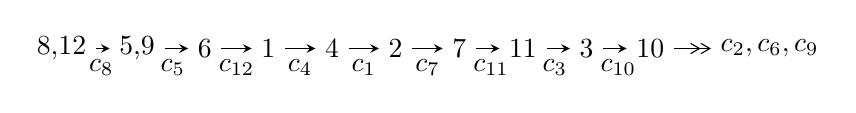
\begin{tikzpicture}[x=23pt, y=7pt]
	% node
	\node (A0) at (-1/8, 0) {8,12};
	\node (A1) at (17/16, 0) {5,9};
	\node (A2) at (17/8, 0) {6};
	\node (A3) at (25/8, 0) {1};
	\node (A4) at (33/8, 0) {4};
	\node (A5) at (41/8, 0) {2};
	\node (A6) at (49/8, 0) {7};
	\node (A7) at (57/8, 0) {11};
	\node (A8) at (65/8, 0) {3};
	\node (A9) at (73/8, 0) {10};
	\node (C1) at (1/2, -1) {$c_{8}$};
	\node (C2) at (13/8, -1) {$c_{5}$};
	\node (C3) at (21/8, -1) {$c_{12}$};
	\node (C4) at (29/8, -1) {$c_{4}$};
	\node (C5) at (37/8, -1) {$c_{1}$};
	\node (C6) at (45/8, -1) {$c_{7}$};
	\node (C7) at (53/8, -1) {$c_{11}$};
	\node (C8) at (61/8, -1) {$c_{3}$};
	\node (C9) at (69/8, -1) {$c_{10}$};
	\node (A10) at (11, 0) {$c_{2},c_{6},c_{9}$};

	% edge
	\draw[->,>=stealth]	
	(A0) edge (A1) (A1) edge (A2) (A2) edge (A3) (A3) edge (A4) (A4) edge (A5) (A5) edge (A6) (A6) edge (A7) (A7) edge (A8) (A8) edge (A9) ;
	\draw[->>,>={angle 60}]	
	(A9) edge (A10);
\end{tikzpicture} \\ 

\end{tabular} \\

\footnotetext{
The image of knot diagram is generated by the software ``\textbf{Draw programme}" developed by Andrew Bartholomew(\url{http://www.layer8.co.uk/maths/draw/index.htm\#Running-draw}), where we modified some parts for our purpose(\url{https://github.com/CATsTAILs/LinksPainter}).
}\phantom \\ \newline 
\centering \textbf{Ideals for irreducible components\footnotemark of $X_{\text{par}}$} 
 
\begin{align*}
I^u_{1}&=\langle 
2.03927\times10^{912} u^{159}+1.35894\times10^{912} u^{158}+\cdots+9.34788\times10^{913} b+5.58125\times10^{916},\\
\phantom{I^u_{1}}&\phantom{= \langle  }-9.45580\times10^{916} u^{159}+1.94852\times10^{917} u^{158}+\cdots+4.24557\times10^{917} a+1.74254\times10^{921},\\
\phantom{I^u_{1}}&\phantom{= \langle  }u^{160}- u^{159}+\cdots-330465 u+18167\rangle \\
I^u_{2}&=\langle 
-1.90847\times10^{34} u^{40}+4.31793\times10^{34} u^{39}+\cdots+1.72831\times10^{34} b+6.15425\times10^{34},\\
\phantom{I^u_{2}}&\phantom{= \langle  }-4.98341\times10^{33} u^{40}-1.50943\times10^{33} u^{39}+\cdots+8.64157\times10^{33} a+4.31559\times10^{34},\;u^{41}-2 u^{40}+\cdots-7 u-1\rangle \\
\\
\end{align*}
\raggedright * 2 irreducible components of $\dim_{\mathbb{C}}=0$, with total 201 representations.\\
\footnotetext{All coefficients of polynomials are rational numbers. But the coefficients are sometimes approximated in decimal forms when there is not enough margin.}
\newpage
\renewcommand{\arraystretch}{1}
\centering \section*{I. $I^u_{1}= \langle 2.04\times10^{912} u^{159}+1.36\times10^{912} u^{158}+\cdots+9.35\times10^{913} b+5.58\times10^{916},\;-9.46\times10^{916} u^{159}+1.95\times10^{917} u^{158}+\cdots+4.25\times10^{917} a+1.74\times10^{921},\;u^{160}- u^{159}+\cdots-330465 u+18167 \rangle$}
\flushleft \textbf{(i) Arc colorings}\\
\begin{tabular}{m{7pt} m{180pt} m{7pt} m{180pt} }
\flushright $a_{8}=$&$\begin{pmatrix}1\\0\end{pmatrix}$ \\
\flushright $a_{12}=$&$\begin{pmatrix}0\\u\end{pmatrix}$ \\
\flushright $a_{5}=$&$\begin{pmatrix}0.222721 u^{159}-0.458952 u^{158}+\cdots+78471.9 u-4104.37\\-0.0218153 u^{159}-0.0145375 u^{158}+\cdots+9981.29 u-597.061\end{pmatrix}$ \\
\flushright $a_{9}=$&$\begin{pmatrix}1\\- u^2\end{pmatrix}$ \\
\flushright $a_{6}=$&$\begin{pmatrix}0.494545 u^{159}-0.943878 u^{158}+\cdots+150603. u-7798.92\\0.267103 u^{159}-0.522995 u^{158}+\cdots+85342.5 u-4468.50\end{pmatrix}$ \\
\flushright $a_{1}=$&$\begin{pmatrix}u\\u\end{pmatrix}$ \\
\flushright $a_{4}=$&$\begin{pmatrix}0.476376 u^{159}-0.920698 u^{158}+\cdots+148967. u-7735.56\\0.231839 u^{159}-0.476284 u^{158}+\cdots+80476.5 u-4228.25\end{pmatrix}$ \\
\flushright $a_{2}=$&$\begin{pmatrix}-0.352143 u^{159}+0.116477 u^{158}+\cdots+69816.5 u-4236.41\\-0.0688601 u^{159}-0.119045 u^{158}+\cdots+61725.5 u-3476.43\end{pmatrix}$ \\
\flushright $a_{7}=$&$\begin{pmatrix}0.0428579 u^{159}-0.445545 u^{158}+\cdots+137371. u-7495.66\\-0.231905 u^{159}-0.0320693 u^{158}+\cdots+82452.8 u-4739.47\end{pmatrix}$ \\
\flushright $a_{11}=$&$\begin{pmatrix}0.227637 u^{159}-0.353886 u^{158}+\cdots+29899.4 u-1386.42\\0.162107 u^{159}-0.459622 u^{158}+\cdots+89079.0 u-4755.16\end{pmatrix}$ \\
\flushright $a_{3}=$&$\begin{pmatrix}0.219745 u^{159}+0.241693 u^{158}+\cdots-120809. u+6892.80\\-0.0572576 u^{159}+0.476848 u^{158}+\cdots-123113. u+6728.65\end{pmatrix}$ \\
\flushright $a_{10}=$&$\begin{pmatrix}0.139410 u^{159}-0.461545 u^{158}+\cdots+112422. u-6012.46\\0.119660 u^{159}-0.178609 u^{158}+\cdots+27642.6 u-1394.50\end{pmatrix}$\\&\end{tabular}
\flushleft \textbf{(ii) Obstruction class $= -1$}\\~\\
\flushleft \textbf{(iii) Cusp Shapes $= -0.237922 u^{159}-0.155452 u^{158}+\cdots+121749. u-6907.25$}\\~\\
\newpage\renewcommand{\arraystretch}{1}
\flushleft \textbf{(iv) u-Polynomials at the component}\newline \\
\begin{tabular}{m{50pt}|m{274pt}}
Crossings & \hspace{64pt}u-Polynomials at each crossing \\
\hline $$\begin{aligned}c_{1},c_{4}\end{aligned}$$&$\begin{aligned}
&u^{160}+4 u^{159}+\cdots-7828 u+1444
\end{aligned}$\\
\hline $$\begin{aligned}c_{2}\end{aligned}$$&$\begin{aligned}
&u^{160}+3 u^{159}+\cdots+341146 u+46381
\end{aligned}$\\
\hline $$\begin{aligned}c_{3}\end{aligned}$$&$\begin{aligned}
&u^{160}-18 u^{158}+\cdots+706845372 u+100225917
\end{aligned}$\\
\hline $$\begin{aligned}c_{5},c_{9}\end{aligned}$$&$\begin{aligned}
&u^{160}+2 u^{159}+\cdots+6873 u+279
\end{aligned}$\\
\hline $$\begin{aligned}c_{6}\end{aligned}$$&$\begin{aligned}
&u^{160}+8 u^{159}+\cdots+40554 u+6463
\end{aligned}$\\
\hline $$\begin{aligned}c_{7}\end{aligned}$$&$\begin{aligned}
&u^{160}+2 u^{159}+\cdots+528175038798 u+68942737333
\end{aligned}$\\
\hline $$\begin{aligned}c_{8},c_{12}\end{aligned}$$&$\begin{aligned}
&u^{160}+u^{159}+\cdots+330465 u+18167
\end{aligned}$\\
\hline $$\begin{aligned}c_{10}\end{aligned}$$&$\begin{aligned}
&u^{160}-3 u^{159}+\cdots+23 u+19
\end{aligned}$\\
\hline $$\begin{aligned}c_{11}\end{aligned}$$&$\begin{aligned}
&u^{160}-28 u^{158}+\cdots-135828304 u+2699248
\end{aligned}$\\
\hline
\end{tabular}\\~\\
\newpage\renewcommand{\arraystretch}{1}
\flushleft \textbf{(v) Riley Polynomials at the component}\newline \\
\begin{tabular}{m{50pt}|m{274pt}}
Crossings & \hspace{64pt}Riley Polynomials at each crossing \\
\hline $$\begin{aligned}c_{1},c_{4}\end{aligned}$$&$\begin{aligned}
&y^{160}+94 y^{159}+\cdots+135556944 y+2085136
\end{aligned}$\\
\hline $$\begin{aligned}c_{2}\end{aligned}$$&$\begin{aligned}
&y^{160}+55 y^{159}+\cdots+289002611650 y+2151197161
\end{aligned}$\\
\hline $$\begin{aligned}c_{3}\end{aligned}$$&$\begin{aligned}
&y^{160}-36 y^{159}+\cdots+235215438020548344 y+10045234438490889
\end{aligned}$\\
\hline $$\begin{aligned}c_{5},c_{9}\end{aligned}$$&$\begin{aligned}
&y^{160}-148 y^{159}+\cdots-15857325 y+77841
\end{aligned}$\\
\hline $$\begin{aligned}c_{6}\end{aligned}$$&$\begin{aligned}
&y^{160}-38 y^{159}+\cdots+4276709054 y+41770369
\end{aligned}$\\
\hline $$\begin{aligned}c_{7}\end{aligned}$$&$\begin{aligned}
&y^{160}+80 y^{159}+\cdots+2.79\times10^{23} y+4.75\times10^{21}
\end{aligned}$\\
\hline $$\begin{aligned}c_{8},c_{12}\end{aligned}$$&$\begin{aligned}
&y^{160}+105 y^{159}+\cdots+15360514711 y+330039889
\end{aligned}$\\
\hline $$\begin{aligned}c_{10}\end{aligned}$$&$\begin{aligned}
&y^{160}+13 y^{159}+\cdots+34469 y+361
\end{aligned}$\\
\hline $$\begin{aligned}c_{11}\end{aligned}$$&$\begin{aligned}
&y^{160}-56 y^{159}+\cdots-10507054762812928 y+7285939765504
\end{aligned}$\\
\hline
\end{tabular}\\~\\
\newpage\flushleft \textbf{(vi) Complex Volumes and Cusp Shapes}
$$\begin{array}{c|c|c}  
\text{Solutions to }I^u_{1}& \I (\text{vol} + \sqrt{-1}CS) & \text{Cusp shape}\\
 \hline 
\begin{aligned}
u &= \phantom{-}0.771319 + 0.637206 I \\
a &= -0.878331 + 0.862171 I \\
b &= -0.484648 + 1.116990 I\end{aligned}
 & -5.69397 + 1.50187 I & \phantom{-0.000000 } 0 \\ \hline\begin{aligned}
u &= \phantom{-}0.771319 - 0.637206 I \\
a &= -0.878331 - 0.862171 I \\
b &= -0.484648 - 1.116990 I\end{aligned}
 & -5.69397 - 1.50187 I & \phantom{-0.000000 } 0 \\ \hline\begin{aligned}
u &= \phantom{-}0.022733 + 1.003480 I \\
a &= -0.261812 + 0.374866 I \\
b &= -1.33271 + 0.93030 I\end{aligned}
 & -1.67760 - 2.03203 I & \phantom{-0.000000 } 0 \\ \hline\begin{aligned}
u &= \phantom{-}0.022733 - 1.003480 I \\
a &= -0.261812 - 0.374866 I \\
b &= -1.33271 - 0.93030 I\end{aligned}
 & -1.67760 + 2.03203 I & \phantom{-0.000000 } 0 \\ \hline\begin{aligned}
u &= \phantom{-}0.929840 + 0.382995 I \\
a &= \phantom{-}0.280467 - 0.907021 I \\
b &= \phantom{-}0.386885 + 0.388981 I\end{aligned}
 & -0.85757 + 4.99990 I & \phantom{-0.000000 } 0 \\ \hline\begin{aligned}
u &= \phantom{-}0.929840 - 0.382995 I \\
a &= \phantom{-}0.280467 + 0.907021 I \\
b &= \phantom{-}0.386885 - 0.388981 I\end{aligned}
 & -0.85757 - 4.99990 I & \phantom{-0.000000 } 0 \\ \hline\begin{aligned}
u &= -0.212329 + 0.970022 I \\
a &= \phantom{-}0.323258 - 0.821506 I \\
b &= -0.021983 - 1.119710 I\end{aligned}
 & -0.84365 - 1.77714 I & \phantom{-0.000000 } 0 \\ \hline\begin{aligned}
u &= -0.212329 - 0.970022 I \\
a &= \phantom{-}0.323258 + 0.821506 I \\
b &= -0.021983 + 1.119710 I\end{aligned}
 & -0.84365 + 1.77714 I & \phantom{-0.000000 } 0 \\ \hline\begin{aligned}
u &= \phantom{-}0.986506 + 0.228196 I \\
a &= -0.749902 - 0.866777 I \\
b &= -0.008395 + 0.163431 I\end{aligned}
 & \phantom{-}1.91050 - 8.98963 I & \phantom{-0.000000 } 0 \\ \hline\begin{aligned}
u &= \phantom{-}0.986506 - 0.228196 I \\
a &= -0.749902 + 0.866777 I \\
b &= -0.008395 - 0.163431 I\end{aligned}
 & \phantom{-}1.91050 + 8.98963 I & \phantom{-0.000000 } 0\\
 \hline 
 \end{array}$$\newpage$$\begin{array}{c|c|c}  
\text{Solutions to }I^u_{1}& \I (\text{vol} + \sqrt{-1}CS) & \text{Cusp shape}\\
 \hline 
\begin{aligned}
u &= \phantom{-}0.193102 + 1.000310 I \\
a &= -0.812533 - 0.993476 I \\
b &= \phantom{-}0.280883 - 0.869016 I\end{aligned}
 & -3.66078 + 3.86809 I & \phantom{-0.000000 } 0 \\ \hline\begin{aligned}
u &= \phantom{-}0.193102 - 1.000310 I \\
a &= -0.812533 + 0.993476 I \\
b &= \phantom{-}0.280883 + 0.869016 I\end{aligned}
 & -3.66078 - 3.86809 I & \phantom{-0.000000 } 0 \\ \hline\begin{aligned}
u &= \phantom{-}0.019225 + 1.021360 I \\
a &= -1.65040 + 0.08303 I \\
b &= -0.178571 + 0.321455 I\end{aligned}
 & -1.76945 + 2.27520 I & \phantom{-0.000000 } 0 \\ \hline\begin{aligned}
u &= \phantom{-}0.019225 - 1.021360 I \\
a &= -1.65040 - 0.08303 I \\
b &= -0.178571 - 0.321455 I\end{aligned}
 & -1.76945 - 2.27520 I & \phantom{-0.000000 } 0 \\ \hline\begin{aligned}
u &= \phantom{-}0.352108 + 0.968435 I \\
a &= -0.270184 + 0.930458 I \\
b &= \phantom{-}0.10069 + 1.81270 I\end{aligned}
 & -2.83007 + 3.63849 I & \phantom{-0.000000 } 0 \\ \hline\begin{aligned}
u &= \phantom{-}0.352108 - 0.968435 I \\
a &= -0.270184 - 0.930458 I \\
b &= \phantom{-}0.10069 - 1.81270 I\end{aligned}
 & -2.83007 - 3.63849 I & \phantom{-0.000000 } 0 \\ \hline\begin{aligned}
u &= -0.890024 + 0.380460 I \\
a &= \phantom{-}1.018230 + 0.695440 I \\
b &= \phantom{-}0.294141 + 0.585359 I\end{aligned}
 & -6.58434 - 9.09290 I & \phantom{-0.000000 } 0 \\ \hline\begin{aligned}
u &= -0.890024 - 0.380460 I \\
a &= \phantom{-}1.018230 - 0.695440 I \\
b &= \phantom{-}0.294141 - 0.585359 I\end{aligned}
 & -6.58434 + 9.09290 I & \phantom{-0.000000 } 0 \\ \hline\begin{aligned}
u &= -0.311265 + 0.893265 I \\
a &= \phantom{-}0.303539 - 0.351570 I \\
b &= \phantom{-}0.91590 - 1.89089 I\end{aligned}
 & -0.99674 - 5.73801 I & \phantom{-0.000000 } 0 \\ \hline\begin{aligned}
u &= -0.311265 - 0.893265 I \\
a &= \phantom{-}0.303539 + 0.351570 I \\
b &= \phantom{-}0.91590 + 1.89089 I\end{aligned}
 & -0.99674 + 5.73801 I & \phantom{-0.000000 } 0\\
 \hline 
 \end{array}$$\newpage$$\begin{array}{c|c|c}  
\text{Solutions to }I^u_{1}& \I (\text{vol} + \sqrt{-1}CS) & \text{Cusp shape}\\
 \hline 
\begin{aligned}
u &= \phantom{-}0.191161 + 0.919191 I \\
a &= -0.857281 + 0.461508 I \\
b &= \phantom{-}0.34084 + 1.42315 I\end{aligned}
 & -1.25091 + 3.41761 I & \phantom{-0.000000 } 0 \\ \hline\begin{aligned}
u &= \phantom{-}0.191161 - 0.919191 I \\
a &= -0.857281 - 0.461508 I \\
b &= \phantom{-}0.34084 - 1.42315 I\end{aligned}
 & -1.25091 - 3.41761 I & \phantom{-0.000000 } 0 \\ \hline\begin{aligned}
u &= \phantom{-}0.718248 + 0.601639 I \\
a &= \phantom{-}0.038366 + 0.773545 I \\
b &= -0.840793 - 0.160007 I\end{aligned}
 & -1.40727 + 0.32935 I & \phantom{-0.000000 } 0 \\ \hline\begin{aligned}
u &= \phantom{-}0.718248 - 0.601639 I \\
a &= \phantom{-}0.038366 - 0.773545 I \\
b &= -0.840793 + 0.160007 I\end{aligned}
 & -1.40727 - 0.32935 I & \phantom{-0.000000 } 0 \\ \hline\begin{aligned}
u &= \phantom{-}0.928288 + 0.112945 I \\
a &= -0.664201 - 0.576783 I \\
b &= -0.777879 + 0.522774 I\end{aligned}
 & -0.911285 + 0.961081 I & \phantom{-0.000000 } 0 \\ \hline\begin{aligned}
u &= \phantom{-}0.928288 - 0.112945 I \\
a &= -0.664201 + 0.576783 I \\
b &= -0.777879 - 0.522774 I\end{aligned}
 & -0.911285 - 0.961081 I & \phantom{-0.000000 } 0 \\ \hline\begin{aligned}
u &= \phantom{-}0.183121 + 1.063230 I \\
a &= -0.349821 - 0.590510 I \\
b &= \phantom{-}0.48392 - 2.02054 I\end{aligned}
 & -3.96270 + 6.64572 I & \phantom{-0.000000 } 0 \\ \hline\begin{aligned}
u &= \phantom{-}0.183121 - 1.063230 I \\
a &= -0.349821 + 0.590510 I \\
b &= \phantom{-}0.48392 + 2.02054 I\end{aligned}
 & -3.96270 - 6.64572 I & \phantom{-0.000000 } 0 \\ \hline\begin{aligned}
u &= \phantom{-}0.015967 + 1.079850 I \\
a &= \phantom{-}2.28551 - 2.06721 I \\
b &= \phantom{-}1.26758 - 2.36916 I\end{aligned}
 & -6.54296 + 8.08154 I & \phantom{-0.000000 } 0 \\ \hline\begin{aligned}
u &= \phantom{-}0.015967 - 1.079850 I \\
a &= \phantom{-}2.28551 + 2.06721 I \\
b &= \phantom{-}1.26758 + 2.36916 I\end{aligned}
 & -6.54296 - 8.08154 I & \phantom{-0.000000 } 0\\
 \hline 
 \end{array}$$\newpage$$\begin{array}{c|c|c}  
\text{Solutions to }I^u_{1}& \I (\text{vol} + \sqrt{-1}CS) & \text{Cusp shape}\\
 \hline 
\begin{aligned}
u &= \phantom{-}0.113157 + 1.079860 I \\
a &= \phantom{-}0.65497 + 1.87674 I \\
b &= -0.17413 + 2.30420 I\end{aligned}
 & -7.21594 + 1.18947 I & \phantom{-0.000000 } 0 \\ \hline\begin{aligned}
u &= \phantom{-}0.113157 - 1.079860 I \\
a &= \phantom{-}0.65497 - 1.87674 I \\
b &= -0.17413 - 2.30420 I\end{aligned}
 & -7.21594 - 1.18947 I & \phantom{-0.000000 } 0 \\ \hline\begin{aligned}
u &= \phantom{-}0.388061 + 1.028440 I \\
a &= -0.161710 - 0.637116 I \\
b &= -1.06523 - 1.31134 I\end{aligned}
 & \phantom{-}2.86422 - 0.13213 I & \phantom{-0.000000 } 0 \\ \hline\begin{aligned}
u &= \phantom{-}0.388061 - 1.028440 I \\
a &= -0.161710 + 0.637116 I \\
b &= -1.06523 + 1.31134 I\end{aligned}
 & \phantom{-}2.86422 + 0.13213 I & \phantom{-0.000000 } 0 \\ \hline\begin{aligned}
u &= -1.082460 + 0.228095 I \\
a &= -0.956574 - 0.173480 I \\
b &= -0.150511 - 0.256263 I\end{aligned}
 & -5.18712 + 1.04076 I & \phantom{-0.000000 } 0 \\ \hline\begin{aligned}
u &= -1.082460 - 0.228095 I \\
a &= -0.956574 + 0.173480 I \\
b &= -0.150511 + 0.256263 I\end{aligned}
 & -5.18712 - 1.04076 I & \phantom{-0.000000 } 0 \\ \hline\begin{aligned}
u &= -0.048192 + 1.112590 I \\
a &= \phantom{-}0.446482 - 0.450424 I \\
b &= -1.45862 - 1.10483 I\end{aligned}
 & -5.73005 - 5.75625 I & \phantom{-0.000000 } 0 \\ \hline\begin{aligned}
u &= -0.048192 - 1.112590 I \\
a &= \phantom{-}0.446482 + 0.450424 I \\
b &= -1.45862 + 1.10483 I\end{aligned}
 & -5.73005 + 5.75625 I & \phantom{-0.000000 } 0 \\ \hline\begin{aligned}
u &= -0.339140 + 1.062200 I \\
a &= -1.24875 - 1.35121 I \\
b &= -0.42773 - 1.95657 I\end{aligned}
 & -2.54983 - 6.54010 I & \phantom{-0.000000 } 0 \\ \hline\begin{aligned}
u &= -0.339140 - 1.062200 I \\
a &= -1.24875 + 1.35121 I \\
b &= -0.42773 + 1.95657 I\end{aligned}
 & -2.54983 + 6.54010 I & \phantom{-0.000000 } 0\\
 \hline 
 \end{array}$$\newpage$$\begin{array}{c|c|c}  
\text{Solutions to }I^u_{1}& \I (\text{vol} + \sqrt{-1}CS) & \text{Cusp shape}\\
 \hline 
\begin{aligned}
u &= -1.093970 + 0.225847 I \\
a &= \phantom{-}0.535300 - 0.544148 I \\
b &= \phantom{-}0.263158 + 0.404730 I\end{aligned}
 & \phantom{-}4.83225 - 0.41382 I & \phantom{-0.000000 } 0 \\ \hline\begin{aligned}
u &= -1.093970 - 0.225847 I \\
a &= \phantom{-}0.535300 + 0.544148 I \\
b &= \phantom{-}0.263158 - 0.404730 I\end{aligned}
 & \phantom{-}4.83225 + 0.41382 I & \phantom{-0.000000 } 0 \\ \hline\begin{aligned}
u &= -0.079655 + 0.878752 I \\
a &= \phantom{-}0.79266 + 2.49745 I \\
b &= \phantom{-}1.58996 + 2.35499 I\end{aligned}
 & -5.66263 - 8.18748 I & \phantom{-0.000000 } 0 \\ \hline\begin{aligned}
u &= -0.079655 - 0.878752 I \\
a &= \phantom{-}0.79266 - 2.49745 I \\
b &= \phantom{-}1.58996 - 2.35499 I\end{aligned}
 & -5.66263 + 8.18748 I & \phantom{-0.000000 } 0 \\ \hline\begin{aligned}
u &= \phantom{-}0.051947 + 1.116560 I \\
a &= -1.13100 - 1.98926 I \\
b &= -0.34451 - 2.25191 I\end{aligned}
 & -7.68881 + 0.18170 I & \phantom{-0.000000 } 0 \\ \hline\begin{aligned}
u &= \phantom{-}0.051947 - 1.116560 I \\
a &= -1.13100 + 1.98926 I \\
b &= -0.34451 + 2.25191 I\end{aligned}
 & -7.68881 - 0.18170 I & \phantom{-0.000000 } 0 \\ \hline\begin{aligned}
u &= -0.036738 + 1.119980 I \\
a &= \phantom{-}0.420703 + 0.920641 I \\
b &= -0.93864 + 1.60800 I\end{aligned}
 & -5.15528 - 3.20035 I & \phantom{-0.000000 } 0 \\ \hline\begin{aligned}
u &= -0.036738 - 1.119980 I \\
a &= \phantom{-}0.420703 - 0.920641 I \\
b &= -0.93864 - 1.60800 I\end{aligned}
 & -5.15528 + 3.20035 I & \phantom{-0.000000 } 0 \\ \hline\begin{aligned}
u &= -0.471836 + 1.034540 I \\
a &= \phantom{-}0.223447 - 0.891094 I \\
b &= \phantom{-}0.82444 - 1.16768 I\end{aligned}
 & \phantom{-}0.37134 - 1.55621 I & \phantom{-0.000000 } 0 \\ \hline\begin{aligned}
u &= -0.471836 - 1.034540 I \\
a &= \phantom{-}0.223447 + 0.891094 I \\
b &= \phantom{-}0.82444 + 1.16768 I\end{aligned}
 & \phantom{-}0.37134 + 1.55621 I & \phantom{-0.000000 } 0\\
 \hline 
 \end{array}$$\newpage$$\begin{array}{c|c|c}  
\text{Solutions to }I^u_{1}& \I (\text{vol} + \sqrt{-1}CS) & \text{Cusp shape}\\
 \hline 
\begin{aligned}
u &= -0.793344 + 0.332222 I \\
a &= -1.57013 + 0.37692 I \\
b &= -0.687251 - 0.912052 I\end{aligned}
 & -0.10292 + 4.82677 I & \phantom{-0.000000 } 0 \\ \hline\begin{aligned}
u &= -0.793344 - 0.332222 I \\
a &= -1.57013 - 0.37692 I \\
b &= -0.687251 + 0.912052 I\end{aligned}
 & -0.10292 - 4.82677 I & \phantom{-0.000000 } 0 \\ \hline\begin{aligned}
u &= -0.788394 + 0.301425 I \\
a &= \phantom{-}0.866249 - 0.959882 I \\
b &= -0.0250898 - 0.0834574 I\end{aligned}
 & \phantom{-}0.756316 - 0.261149 I & \phantom{-0.000000 } 0 \\ \hline\begin{aligned}
u &= -0.788394 - 0.301425 I \\
a &= \phantom{-}0.866249 + 0.959882 I \\
b &= -0.0250898 + 0.0834574 I\end{aligned}
 & \phantom{-}0.756316 + 0.261149 I & \phantom{-0.000000 } 0 \\ \hline\begin{aligned}
u &= \phantom{-}0.312537 + 1.119230 I \\
a &= \phantom{-}0.440519 + 1.271460 I \\
b &= \phantom{-}1.32997 + 1.85254 I\end{aligned}
 & \phantom{-}1.65273 + 6.18718 I & \phantom{-0.000000 } 0 \\ \hline\begin{aligned}
u &= \phantom{-}0.312537 - 1.119230 I \\
a &= \phantom{-}0.440519 - 1.271460 I \\
b &= \phantom{-}1.32997 - 1.85254 I\end{aligned}
 & \phantom{-}1.65273 - 6.18718 I & \phantom{-0.000000 } 0 \\ \hline\begin{aligned}
u &= -0.485941 + 0.677045 I \\
a &= \phantom{-}1.129400 - 0.792715 I \\
b &= -0.548995 - 0.549939 I\end{aligned}
 & -0.47469 + 2.27310 I & \phantom{-0.000000 } 0 \\ \hline\begin{aligned}
u &= -0.485941 - 0.677045 I \\
a &= \phantom{-}1.129400 + 0.792715 I \\
b &= -0.548995 + 0.549939 I\end{aligned}
 & -0.47469 - 2.27310 I & \phantom{-0.000000 } 0 \\ \hline\begin{aligned}
u &= -0.789850 + 0.225465 I \\
a &= \phantom{-}0.284065 - 1.160750 I \\
b &= \phantom{-}0.252789 + 0.295295 I\end{aligned}
 & \phantom{-}2.68987 - 3.10360 I & \phantom{-0.000000 } 0 \\ \hline\begin{aligned}
u &= -0.789850 - 0.225465 I \\
a &= \phantom{-}0.284065 + 1.160750 I \\
b &= \phantom{-}0.252789 - 0.295295 I\end{aligned}
 & \phantom{-}2.68987 + 3.10360 I & \phantom{-0.000000 } 0\\
 \hline 
 \end{array}$$\newpage$$\begin{array}{c|c|c}  
\text{Solutions to }I^u_{1}& \I (\text{vol} + \sqrt{-1}CS) & \text{Cusp shape}\\
 \hline 
\begin{aligned}
u &= -0.146895 + 1.195160 I \\
a &= -0.435482 + 0.462232 I \\
b &= -0.636280 + 1.194530 I\end{aligned}
 & -3.64158 - 2.72765 I & \phantom{-0.000000 } 0 \\ \hline\begin{aligned}
u &= -0.146895 - 1.195160 I \\
a &= -0.435482 - 0.462232 I \\
b &= -0.636280 - 1.194530 I\end{aligned}
 & -3.64158 + 2.72765 I & \phantom{-0.000000 } 0 \\ \hline\begin{aligned}
u &= \phantom{-}0.038248 + 1.203750 I \\
a &= -0.127547 + 0.769202 I \\
b &= -0.13411 + 1.96529 I\end{aligned}
 & -5.58598 + 0.17460 I & \phantom{-0.000000 } 0 \\ \hline\begin{aligned}
u &= \phantom{-}0.038248 - 1.203750 I \\
a &= -0.127547 - 0.769202 I \\
b &= -0.13411 - 1.96529 I\end{aligned}
 & -5.58598 - 0.17460 I & \phantom{-0.000000 } 0 \\ \hline\begin{aligned}
u &= -0.507786 + 1.096330 I \\
a &= \phantom{-}0.431517 - 0.787097 I \\
b &= \phantom{-}0.87693 - 1.77504 I\end{aligned}
 & -1.63186 - 4.52471 I & \phantom{-0.000000 } 0 \\ \hline\begin{aligned}
u &= -0.507786 - 1.096330 I \\
a &= \phantom{-}0.431517 + 0.787097 I \\
b &= \phantom{-}0.87693 + 1.77504 I\end{aligned}
 & -1.63186 + 4.52471 I & \phantom{-0.000000 } 0 \\ \hline\begin{aligned}
u &= \phantom{-}0.385112 + 1.145430 I \\
a &= \phantom{-}0.736869 - 0.874360 I \\
b &= \phantom{-}0.18404 - 1.45269 I\end{aligned}
 & -3.82526 - 1.22877 I & \phantom{-0.000000 } 0 \\ \hline\begin{aligned}
u &= \phantom{-}0.385112 - 1.145430 I \\
a &= \phantom{-}0.736869 + 0.874360 I \\
b &= \phantom{-}0.18404 + 1.45269 I\end{aligned}
 & -3.82526 + 1.22877 I & \phantom{-0.000000 } 0 \\ \hline\begin{aligned}
u &= \phantom{-}0.003758 + 1.224780 I \\
a &= -0.325431 + 0.476596 I \\
b &= \phantom{-}0.96253 + 1.13630 I\end{aligned}
 & -5.74021 + 3.13154 I & \phantom{-0.000000 } 0 \\ \hline\begin{aligned}
u &= \phantom{-}0.003758 - 1.224780 I \\
a &= -0.325431 - 0.476596 I \\
b &= \phantom{-}0.96253 - 1.13630 I\end{aligned}
 & -5.74021 - 3.13154 I & \phantom{-0.000000 } 0\\
 \hline 
 \end{array}$$\newpage$$\begin{array}{c|c|c}  
\text{Solutions to }I^u_{1}& \I (\text{vol} + \sqrt{-1}CS) & \text{Cusp shape}\\
 \hline 
\begin{aligned}
u &= -0.170381 + 0.737075 I \\
a &= \phantom{-}0.45292 + 1.81818 I \\
b &= -0.29703 + 1.94984 I\end{aligned}
 & -1.22555 + 3.89889 I & \phantom{-0.000000 } 0 \\ \hline\begin{aligned}
u &= -0.170381 - 0.737075 I \\
a &= \phantom{-}0.45292 - 1.81818 I \\
b &= -0.29703 - 1.94984 I\end{aligned}
 & -1.22555 - 3.89889 I & \phantom{-0.000000 } 0 \\ \hline\begin{aligned}
u &= \phantom{-}0.248270 + 0.714425 I \\
a &= -0.015415 - 0.474095 I \\
b &= -1.050810 - 0.319934 I\end{aligned}
 & -1.44296 - 1.53470 I & \phantom{-0.000000 } 0 \\ \hline\begin{aligned}
u &= \phantom{-}0.248270 - 0.714425 I \\
a &= -0.015415 + 0.474095 I \\
b &= -1.050810 + 0.319934 I\end{aligned}
 & -1.44296 + 1.53470 I & \phantom{-0.000000 } 0 \\ \hline\begin{aligned}
u &= \phantom{-}0.701027 + 0.271853 I \\
a &= \phantom{-}0.938700 + 0.760765 I \\
b &= -0.158470 - 0.480526 I\end{aligned}
 & \phantom{-}1.33311 - 3.17107 I & \phantom{-0.000000 } 0 \\ \hline\begin{aligned}
u &= \phantom{-}0.701027 - 0.271853 I \\
a &= \phantom{-}0.938700 - 0.760765 I \\
b &= -0.158470 + 0.480526 I\end{aligned}
 & \phantom{-}1.33311 + 3.17107 I & \phantom{-0.000000 } 0 \\ \hline\begin{aligned}
u &= \phantom{-}0.424720 + 1.183200 I \\
a &= \phantom{-}0.016532 + 0.971665 I \\
b &= \phantom{-}0.84910 + 1.86937 I\end{aligned}
 & -1.53801 + 7.47985 I & \phantom{-0.000000 } 0 \\ \hline\begin{aligned}
u &= \phantom{-}0.424720 - 1.183200 I \\
a &= \phantom{-}0.016532 - 0.971665 I \\
b &= \phantom{-}0.84910 - 1.86937 I\end{aligned}
 & -1.53801 - 7.47985 I & \phantom{-0.000000 } 0 \\ \hline\begin{aligned}
u &= \phantom{-}1.260680 + 0.052977 I \\
a &= -0.733708 - 0.431970 I \\
b &= -0.338946 + 0.350189 I\end{aligned}
 & -3.93925 - 5.16916 I & \phantom{-0.000000 } 0 \\ \hline\begin{aligned}
u &= \phantom{-}1.260680 - 0.052977 I \\
a &= -0.733708 + 0.431970 I \\
b &= -0.338946 - 0.350189 I\end{aligned}
 & -3.93925 + 5.16916 I & \phantom{-0.000000 } 0\\
 \hline 
 \end{array}$$\newpage$$\begin{array}{c|c|c}  
\text{Solutions to }I^u_{1}& \I (\text{vol} + \sqrt{-1}CS) & \text{Cusp shape}\\
 \hline 
\begin{aligned}
u &= \phantom{-}0.624978 + 0.381968 I \\
a &= -1.30233 + 0.86319 I \\
b &= -0.763440 + 0.814076 I\end{aligned}
 & -5.71505 + 1.46266 I & \phantom{-0.000000 } 0 \\ \hline\begin{aligned}
u &= \phantom{-}0.624978 - 0.381968 I \\
a &= -1.30233 - 0.86319 I \\
b &= -0.763440 - 0.814076 I\end{aligned}
 & -5.71505 - 1.46266 I & \phantom{-0.000000 } 0 \\ \hline\begin{aligned}
u &= -0.448956 + 1.187160 I \\
a &= -0.09626 + 2.00763 I \\
b &= -0.91109 + 2.56937 I\end{aligned}
 & -2.83904 - 9.49173 I & \phantom{-0.000000 } 0 \\ \hline\begin{aligned}
u &= -0.448956 - 1.187160 I \\
a &= -0.09626 - 2.00763 I \\
b &= -0.91109 - 2.56937 I\end{aligned}
 & -2.83904 + 9.49173 I & \phantom{-0.000000 } 0 \\ \hline\begin{aligned}
u &= -1.266150 + 0.203428 I \\
a &= -0.770800 + 0.179739 I \\
b &= -0.199623 - 0.622947 I\end{aligned}
 & -2.65691 + 4.12603 I & \phantom{-0.000000 } 0 \\ \hline\begin{aligned}
u &= -1.266150 - 0.203428 I \\
a &= -0.770800 - 0.179739 I \\
b &= -0.199623 + 0.622947 I\end{aligned}
 & -2.65691 - 4.12603 I & \phantom{-0.000000 } 0 \\ \hline\begin{aligned}
u &= \phantom{-}0.572284 + 0.429818 I \\
a &= -1.05476 - 1.25532 I \\
b &= \phantom{-}0.137410 + 0.259897 I\end{aligned}
 & \phantom{-}4.77299 + 4.00153 I & \phantom{-0.000000 } 0 \\ \hline\begin{aligned}
u &= \phantom{-}0.572284 - 0.429818 I \\
a &= -1.05476 + 1.25532 I \\
b &= \phantom{-}0.137410 - 0.259897 I\end{aligned}
 & \phantom{-}4.77299 - 4.00153 I & \phantom{-0.000000 } 0 \\ \hline\begin{aligned}
u &= -1.312040 + 0.004704 I \\
a &= \phantom{-}0.676803 - 0.455758 I \\
b &= \phantom{-}0.290545 + 0.435528 I\end{aligned}
 & -3.6980 + 13.6691 I & \phantom{-0.000000 } 0 \\ \hline\begin{aligned}
u &= -1.312040 - 0.004704 I \\
a &= \phantom{-}0.676803 + 0.455758 I \\
b &= \phantom{-}0.290545 - 0.435528 I\end{aligned}
 & -3.6980 - 13.6691 I & \phantom{-0.000000 } 0\\
 \hline 
 \end{array}$$\newpage$$\begin{array}{c|c|c}  
\text{Solutions to }I^u_{1}& \I (\text{vol} + \sqrt{-1}CS) & \text{Cusp shape}\\
 \hline 
\begin{aligned}
u &= \phantom{-}0.533669 + 1.221510 I \\
a &= -0.357373 - 0.938096 I \\
b &= -1.02542 - 1.85578 I\end{aligned}
 & -1.2187 + 14.4133 I & \phantom{-0.000000 } 0 \\ \hline\begin{aligned}
u &= \phantom{-}0.533669 - 1.221510 I \\
a &= -0.357373 + 0.938096 I \\
b &= -1.02542 + 1.85578 I\end{aligned}
 & -1.2187 - 14.4133 I & \phantom{-0.000000 } 0 \\ \hline\begin{aligned}
u &= -0.367274 + 1.293060 I \\
a &= -0.276160 + 0.782809 I \\
b &= -1.07384 + 1.57529 I\end{aligned}
 & -1.89105 - 7.16268 I & \phantom{-0.000000 } 0 \\ \hline\begin{aligned}
u &= -0.367274 - 1.293060 I \\
a &= -0.276160 - 0.782809 I \\
b &= -1.07384 - 1.57529 I\end{aligned}
 & -1.89105 + 7.16268 I & \phantom{-0.000000 } 0 \\ \hline\begin{aligned}
u &= -0.206745 + 1.329860 I \\
a &= -0.691173 - 0.328586 I \\
b &= -1.068150 - 0.488779 I\end{aligned}
 & -4.49979 - 3.43539 I & \phantom{-0.000000 } 0 \\ \hline\begin{aligned}
u &= -0.206745 - 1.329860 I \\
a &= -0.691173 + 0.328586 I \\
b &= -1.068150 + 0.488779 I\end{aligned}
 & -4.49979 + 3.43539 I & \phantom{-0.000000 } 0 \\ \hline\begin{aligned}
u &= -0.523543 + 1.252300 I \\
a &= \phantom{-}0.319372 - 1.085070 I \\
b &= \phantom{-}0.95238 - 1.66839 I\end{aligned}
 & \phantom{-}1.48788 - 5.16257 I & \phantom{-0.000000 } 0 \\ \hline\begin{aligned}
u &= -0.523543 - 1.252300 I \\
a &= \phantom{-}0.319372 + 1.085070 I \\
b &= \phantom{-}0.95238 + 1.66839 I\end{aligned}
 & \phantom{-}1.48788 + 5.16257 I & \phantom{-0.000000 } 0 \\ \hline\begin{aligned}
u &= \phantom{-}0.366217 + 1.326070 I \\
a &= -0.429611 - 1.018580 I \\
b &= \phantom{-}0.09687 - 1.67663 I\end{aligned}
 & -10.62430 + 5.37850 I & \phantom{-0.000000 } 0 \\ \hline\begin{aligned}
u &= \phantom{-}0.366217 - 1.326070 I \\
a &= -0.429611 + 1.018580 I \\
b &= \phantom{-}0.09687 + 1.67663 I\end{aligned}
 & -10.62430 - 5.37850 I & \phantom{-0.000000 } 0\\
 \hline 
 \end{array}$$\newpage$$\begin{array}{c|c|c}  
\text{Solutions to }I^u_{1}& \I (\text{vol} + \sqrt{-1}CS) & \text{Cusp shape}\\
 \hline 
\begin{aligned}
u &= \phantom{-}0.241300 + 1.357060 I \\
a &= \phantom{-}0.480348 + 1.161640 I \\
b &= \phantom{-}0.23429 + 2.02195 I\end{aligned}
 & -10.27410 + 3.62043 I & \phantom{-0.000000 } 0 \\ \hline\begin{aligned}
u &= \phantom{-}0.241300 - 1.357060 I \\
a &= \phantom{-}0.480348 - 1.161640 I \\
b &= \phantom{-}0.23429 - 2.02195 I\end{aligned}
 & -10.27410 - 3.62043 I & \phantom{-0.000000 } 0 \\ \hline\begin{aligned}
u &= -0.596376 + 1.255710 I \\
a &= -0.002940 + 0.597827 I \\
b &= -0.68621 + 1.27720 I\end{aligned}
 & \phantom{-}0.87079 - 7.02461 I & \phantom{-0.000000 } 0 \\ \hline\begin{aligned}
u &= -0.596376 - 1.255710 I \\
a &= -0.002940 - 0.597827 I \\
b &= -0.68621 - 1.27720 I\end{aligned}
 & \phantom{-}0.87079 + 7.02461 I & \phantom{-0.000000 } 0 \\ \hline\begin{aligned}
u &= \phantom{-}0.070293 + 1.402540 I \\
a &= \phantom{-}1.73238 + 0.14815 I \\
b &= \phantom{-}2.08880 + 0.12438 I\end{aligned}
 & -8.75345 + 5.70112 I & \phantom{-0.000000 } 0 \\ \hline\begin{aligned}
u &= \phantom{-}0.070293 - 1.402540 I \\
a &= \phantom{-}1.73238 - 0.14815 I \\
b &= \phantom{-}2.08880 - 0.12438 I\end{aligned}
 & -8.75345 - 5.70112 I & \phantom{-0.000000 } 0 \\ \hline\begin{aligned}
u &= \phantom{-}0.15398 + 1.40780 I \\
a &= -1.44312 - 1.07283 I \\
b &= -2.01266 - 1.31893 I\end{aligned}
 & -7.92244 + 2.88032 I & \phantom{-0.000000 } 0 \\ \hline\begin{aligned}
u &= \phantom{-}0.15398 - 1.40780 I \\
a &= -1.44312 + 1.07283 I \\
b &= -2.01266 + 1.31893 I\end{aligned}
 & -7.92244 - 2.88032 I & \phantom{-0.000000 } 0 \\ \hline\begin{aligned}
u &= -0.36539 + 1.37089 I \\
a &= \phantom{-}0.368191 - 1.029030 I \\
b &= \phantom{-}0.01615 - 1.88284 I\end{aligned}
 & -11.9011 - 13.4082 I & \phantom{-0.000000 } 0 \\ \hline\begin{aligned}
u &= -0.36539 - 1.37089 I \\
a &= \phantom{-}0.368191 + 1.029030 I \\
b &= \phantom{-}0.01615 + 1.88284 I\end{aligned}
 & -11.9011 + 13.4082 I & \phantom{-0.000000 } 0\\
 \hline 
 \end{array}$$\newpage$$\begin{array}{c|c|c}  
\text{Solutions to }I^u_{1}& \I (\text{vol} + \sqrt{-1}CS) & \text{Cusp shape}\\
 \hline 
\begin{aligned}
u &= \phantom{-}0.55963 + 1.32820 I \\
a &= -0.330042 - 1.188310 I \\
b &= -0.85538 - 1.46121 I\end{aligned}
 & -4.79671 + 4.65674 I & \phantom{-0.000000 } 0 \\ \hline\begin{aligned}
u &= \phantom{-}0.55963 - 1.32820 I \\
a &= -0.330042 + 1.188310 I \\
b &= -0.85538 + 1.46121 I\end{aligned}
 & -4.79671 - 4.65674 I & \phantom{-0.000000 } 0 \\ \hline\begin{aligned}
u &= -1.41738 + 0.26867 I \\
a &= -0.066927 + 0.261952 I \\
b &= \phantom{-}0.157318 - 0.402861 I\end{aligned}
 & \phantom{-}4.32946 + 0.49134 I & \phantom{-0.000000 } 0 \\ \hline\begin{aligned}
u &= -1.41738 - 0.26867 I \\
a &= -0.066927 - 0.261952 I \\
b &= \phantom{-}0.157318 + 0.402861 I\end{aligned}
 & \phantom{-}4.32946 - 0.49134 I & \phantom{-0.000000 } 0 \\ \hline\begin{aligned}
u &= \phantom{-}0.21953 + 1.43065 I \\
a &= \phantom{-}0.972718 + 0.841552 I \\
b &= \phantom{-}1.09866 + 1.28048 I\end{aligned}
 & -8.47419 + 5.75201 I & \phantom{-0.000000 } 0 \\ \hline\begin{aligned}
u &= \phantom{-}0.21953 - 1.43065 I \\
a &= \phantom{-}0.972718 - 0.841552 I \\
b &= \phantom{-}1.09866 - 1.28048 I\end{aligned}
 & -8.47419 - 5.75201 I & \phantom{-0.000000 } 0 \\ \hline\begin{aligned}
u &= -0.461117 + 0.297405 I \\
a &= \phantom{-}0.673049 - 0.745905 I \\
b &= \phantom{-}0.189026 - 0.287413 I\end{aligned}
 & \phantom{-}0.877529 - 1.031680 I & \phantom{-0.000000 } 0 \\ \hline\begin{aligned}
u &= -0.461117 - 0.297405 I \\
a &= \phantom{-}0.673049 + 0.745905 I \\
b &= \phantom{-}0.189026 + 0.287413 I\end{aligned}
 & \phantom{-}0.877529 + 1.031680 I & \phantom{-0.000000 } 0 \\ \hline\begin{aligned}
u &= \phantom{-}0.476211 + 0.261545 I \\
a &= \phantom{-}1.73825 - 1.23491 I \\
b &= \phantom{-}0.677847 - 0.231017 I\end{aligned}
 & -5.14917 + 0.94616 I & \phantom{-0.000000 } 0 \\ \hline\begin{aligned}
u &= \phantom{-}0.476211 - 0.261545 I \\
a &= \phantom{-}1.73825 + 1.23491 I \\
b &= \phantom{-}0.677847 + 0.231017 I\end{aligned}
 & -5.14917 - 0.94616 I & \phantom{-0.000000 } 0\\
 \hline 
 \end{array}$$\newpage$$\begin{array}{c|c|c}  
\text{Solutions to }I^u_{1}& \I (\text{vol} + \sqrt{-1}CS) & \text{Cusp shape}\\
 \hline 
\begin{aligned}
u &= -0.37846 + 1.41696 I \\
a &= -0.203143 + 0.912738 I \\
b &= \phantom{-}0.05857 + 1.74835 I\end{aligned}
 & -10.61080 - 4.04474 I & \phantom{-0.000000 } 0 \\ \hline\begin{aligned}
u &= -0.37846 - 1.41696 I \\
a &= -0.203143 - 0.912738 I \\
b &= \phantom{-}0.05857 - 1.74835 I\end{aligned}
 & -10.61080 + 4.04474 I & \phantom{-0.000000 } 0 \\ \hline\begin{aligned}
u &= -0.30689 + 1.45855 I \\
a &= -0.374028 + 0.577175 I \\
b &= \phantom{-}0.170856 + 1.068930 I\end{aligned}
 & -8.82195 - 1.43934 I & \phantom{-0.000000 } 0 \\ \hline\begin{aligned}
u &= -0.30689 - 1.45855 I \\
a &= -0.374028 - 0.577175 I \\
b &= \phantom{-}0.170856 - 1.068930 I\end{aligned}
 & -8.82195 + 1.43934 I & \phantom{-0.000000 } 0 \\ \hline\begin{aligned}
u &= \phantom{-}0.380278 + 0.330357 I \\
a &= -0.0621875 + 0.0343678 I \\
b &= -1.010000 - 0.196503 I\end{aligned}
 & -1.85407 - 1.13333 I & \phantom{-0.000000 } 0 \\ \hline\begin{aligned}
u &= \phantom{-}0.380278 - 0.330357 I \\
a &= -0.0621875 - 0.0343678 I \\
b &= -1.010000 + 0.196503 I\end{aligned}
 & -1.85407 + 1.13333 I & \phantom{-0.000000 } 0 \\ \hline\begin{aligned}
u &= -0.67450 + 1.33711 I \\
a &= \phantom{-}0.065441 + 0.933565 I \\
b &= -0.16160 + 1.62092 I\end{aligned}
 & -8.46875 - 7.38395 I & \phantom{-0.000000 } 0 \\ \hline\begin{aligned}
u &= -0.67450 - 1.33711 I \\
a &= \phantom{-}0.065441 - 0.933565 I \\
b &= -0.16160 - 1.62092 I\end{aligned}
 & -8.46875 + 7.38395 I & \phantom{-0.000000 } 0 \\ \hline\begin{aligned}
u &= \phantom{-}0.251192 + 0.432476 I \\
a &= \phantom{-}3.02441 + 0.67825 I \\
b &= \phantom{-}0.460875 - 0.371861 I\end{aligned}
 & \phantom{-}4.05011 - 3.41466 I & \phantom{-}11.3240 - 10.5501 I \\ \hline\begin{aligned}
u &= \phantom{-}0.251192 - 0.432476 I \\
a &= \phantom{-}3.02441 - 0.67825 I \\
b &= \phantom{-}0.460875 + 0.371861 I\end{aligned}
 & \phantom{-}4.05011 + 3.41466 I & \phantom{-}11.3240 + 10.5501 I\\
 \hline 
 \end{array}$$\newpage$$\begin{array}{c|c|c}  
\text{Solutions to }I^u_{1}& \I (\text{vol} + \sqrt{-1}CS) & \text{Cusp shape}\\
 \hline 
\begin{aligned}
u &= \phantom{-}0.72800 + 1.31378 I \\
a &= \phantom{-}0.255955 - 1.010980 I \\
b &= -0.20136 - 1.59818 I\end{aligned}
 & -7.94125 + 4.99424 I & \phantom{-0.000000 } 0 \\ \hline\begin{aligned}
u &= \phantom{-}0.72800 - 1.31378 I \\
a &= \phantom{-}0.255955 + 1.010980 I \\
b &= -0.20136 + 1.59818 I\end{aligned}
 & -7.94125 - 4.99424 I & \phantom{-0.000000 } 0 \\ \hline\begin{aligned}
u &= \phantom{-}0.09550 + 1.50794 I \\
a &= \phantom{-}0.363142 - 0.345910 I \\
b &= \phantom{-}0.865257 - 0.533965 I\end{aligned}
 & -4.32371 - 4.70566 I & \phantom{-0.000000 } 0 \\ \hline\begin{aligned}
u &= \phantom{-}0.09550 - 1.50794 I \\
a &= \phantom{-}0.363142 + 0.345910 I \\
b &= \phantom{-}0.865257 + 0.533965 I\end{aligned}
 & -4.32371 + 4.70566 I & \phantom{-0.000000 } 0 \\ \hline\begin{aligned}
u &= \phantom{-}0.58023 + 1.39854 I \\
a &= -0.333307 - 1.219160 I \\
b &= -0.88707 - 1.92612 I\end{aligned}
 & -8.2640 + 11.5613 I & \phantom{-0.000000 } 0 \\ \hline\begin{aligned}
u &= \phantom{-}0.58023 - 1.39854 I \\
a &= -0.333307 + 1.219160 I \\
b &= -0.88707 + 1.92612 I\end{aligned}
 & -8.2640 - 11.5613 I & \phantom{-0.000000 } 0 \\ \hline\begin{aligned}
u &= -0.63153 + 1.38691 I \\
a &= -0.043485 + 1.149410 I \\
b &= -0.68966 + 1.92416 I\end{aligned}
 & -6.51467 - 10.82670 I & \phantom{-0.000000 } 0 \\ \hline\begin{aligned}
u &= -0.63153 - 1.38691 I \\
a &= -0.043485 - 1.149410 I \\
b &= -0.68966 - 1.92416 I\end{aligned}
 & -6.51467 + 10.82670 I & \phantom{-0.000000 } 0 \\ \hline\begin{aligned}
u &= -0.58847 + 1.41912 I \\
a &= \phantom{-}0.299592 - 1.221220 I \\
b &= \phantom{-}0.94418 - 1.96269 I\end{aligned}
 & -8.2027 - 20.2163 I & \phantom{-0.000000 } 0 \\ \hline\begin{aligned}
u &= -0.58847 - 1.41912 I \\
a &= \phantom{-}0.299592 + 1.221220 I \\
b &= \phantom{-}0.94418 + 1.96269 I\end{aligned}
 & -8.2027 + 20.2163 I & \phantom{-0.000000 } 0\\
 \hline 
 \end{array}$$\newpage$$\begin{array}{c|c|c}  
\text{Solutions to }I^u_{1}& \I (\text{vol} + \sqrt{-1}CS) & \text{Cusp shape}\\
 \hline 
\begin{aligned}
u &= \phantom{-}0.45748 + 1.46989 I \\
a &= \phantom{-}0.502954 + 1.174800 I \\
b &= \phantom{-}1.19330 + 1.83621 I\end{aligned}
 & -6.61253 + 10.16070 I & \phantom{-0.000000 } 0 \\ \hline\begin{aligned}
u &= \phantom{-}0.45748 - 1.46989 I \\
a &= \phantom{-}0.502954 - 1.174800 I \\
b &= \phantom{-}1.19330 - 1.83621 I\end{aligned}
 & -6.61253 - 10.16070 I & \phantom{-0.000000 } 0 \\ \hline\begin{aligned}
u &= \phantom{-}0.310820 + 0.308657 I \\
a &= \phantom{-}0.03495 - 2.33270 I \\
b &= \phantom{-}0.780590 - 0.100267 I\end{aligned}
 & -3.00308 + 3.55964 I & -9.14461 - 7.54866 I \\ \hline\begin{aligned}
u &= \phantom{-}0.310820 - 0.308657 I \\
a &= \phantom{-}0.03495 + 2.33270 I \\
b &= \phantom{-}0.780590 + 0.100267 I\end{aligned}
 & -3.00308 - 3.55964 I & -9.14461 + 7.54866 I \\ \hline\begin{aligned}
u &= \phantom{-}0.40246 + 1.51659 I \\
a &= -0.239997 - 0.600596 I \\
b &= \phantom{-}0.165277 - 0.828672 I\end{aligned}
 & -9.47807 + 1.09420 I & \phantom{-0.000000 } 0 \\ \hline\begin{aligned}
u &= \phantom{-}0.40246 - 1.51659 I \\
a &= -0.239997 + 0.600596 I \\
b &= \phantom{-}0.165277 + 0.828672 I\end{aligned}
 & -9.47807 - 1.09420 I & \phantom{-0.000000 } 0 \\ \hline\begin{aligned}
u &= \phantom{-}0.323168 + 0.276129 I \\
a &= \phantom{-}1.28688 - 0.66363 I \\
b &= -0.231336 - 0.218065 I\end{aligned}
 & -1.35697 - 0.78698 I & -4.61483 + 0. I\phantom{ +0.000000I} \\ \hline\begin{aligned}
u &= \phantom{-}0.323168 - 0.276129 I \\
a &= \phantom{-}1.28688 + 0.66363 I \\
b &= -0.231336 + 0.218065 I\end{aligned}
 & -1.35697 + 0.78698 I & -4.61483 + 0. I\phantom{ +0.000000I} \\ \hline\begin{aligned}
u &= -0.83498 + 1.34845 I \\
a &= -0.258565 - 0.759130 I \\
b &= \phantom{-}0.030686 - 1.336400 I\end{aligned}
 & -8.79556 + 2.43577 I & \phantom{-0.000000 } 0 \\ \hline\begin{aligned}
u &= -0.83498 - 1.34845 I \\
a &= -0.258565 + 0.759130 I \\
b &= \phantom{-}0.030686 + 1.336400 I\end{aligned}
 & -8.79556 - 2.43577 I & \phantom{-0.000000 } 0\\
 \hline 
 \end{array}$$\newpage$$\begin{array}{c|c|c}  
\text{Solutions to }I^u_{1}& \I (\text{vol} + \sqrt{-1}CS) & \text{Cusp shape}\\
 \hline 
\begin{aligned}
u &= \phantom{-}0.342694 + 0.060758 I \\
a &= -1.91156 + 1.21730 I \\
b &= \phantom{-}0.043009 + 0.951918 I\end{aligned}
 & -1.28324 + 4.45890 I & -2.67295 - 6.46132 I \\ \hline\begin{aligned}
u &= \phantom{-}0.342694 - 0.060758 I \\
a &= -1.91156 - 1.21730 I \\
b &= \phantom{-}0.043009 - 0.951918 I\end{aligned}
 & -1.28324 - 4.45890 I & -2.67295 + 6.46132 I \\ \hline\begin{aligned}
u &= \phantom{-}0.66432 + 1.58517 I \\
a &= \phantom{-}0.258644 + 0.807061 I \\
b &= \phantom{-}0.82952 + 1.32959 I\end{aligned}
 & -4.38043 + 9.74516 I & \phantom{-0.000000 } 0 \\ \hline\begin{aligned}
u &= \phantom{-}0.66432 - 1.58517 I \\
a &= \phantom{-}0.258644 - 0.807061 I \\
b &= \phantom{-}0.82952 - 1.32959 I\end{aligned}
 & -4.38043 - 9.74516 I & \phantom{-0.000000 } 0 \\ \hline\begin{aligned}
u &= \phantom{-}0.001860 + 0.251704 I \\
a &= -3.06934 + 1.68254 I \\
b &= \phantom{-}1.181710 - 0.337517 I\end{aligned}
 & -3.45857 + 5.38370 I & -2.31636 - 2.96404 I \\ \hline\begin{aligned}
u &= \phantom{-}0.001860 - 0.251704 I \\
a &= -3.06934 - 1.68254 I \\
b &= \phantom{-}1.181710 + 0.337517 I\end{aligned}
 & -3.45857 - 5.38370 I & -2.31636 + 2.96404 I \\ \hline\begin{aligned}
u &= -0.37870 + 1.73609 I \\
a &= \phantom{-}0.274293 - 0.349257 I \\
b &= -0.149930 - 0.504723 I\end{aligned}
 & -9.42360 + 6.52384 I & \phantom{-0.000000 } 0 \\ \hline\begin{aligned}
u &= -0.37870 - 1.73609 I \\
a &= \phantom{-}0.274293 + 0.349257 I \\
b &= -0.149930 + 0.504723 I\end{aligned}
 & -9.42360 - 6.52384 I & \phantom{-0.000000 } 0 \\ \hline\begin{aligned}
u &= \phantom{-}1.91147 + 0.31167 I \\
a &= \phantom{-}0.337860 + 0.017754 I \\
b &= \phantom{-}0.141213 - 0.437150 I\end{aligned}
 & \phantom{-}0.564712 - 0.995876 I & \phantom{-0.000000 } 0 \\ \hline\begin{aligned}
u &= \phantom{-}1.91147 - 0.31167 I \\
a &= \phantom{-}0.337860 - 0.017754 I \\
b &= \phantom{-}0.141213 + 0.437150 I\end{aligned}
 & \phantom{-}0.564712 + 0.995876 I & \phantom{-0.000000 } 0\\
 \hline 
 \end{array}$$\newpage\newpage\renewcommand{\arraystretch}{1}
\centering \section*{II. $I^u_{2}= \langle -1.91\times10^{34} u^{40}+4.32\times10^{34} u^{39}+\cdots+1.73\times10^{34} b+6.15\times10^{34},\;-4.98\times10^{33} u^{40}-1.51\times10^{33} u^{39}+\cdots+8.64\times10^{33} a+4.32\times10^{34},\;u^{41}-2 u^{40}+\cdots-7 u-1 \rangle$}
\flushleft \textbf{(i) Arc colorings}\\
\begin{tabular}{m{7pt} m{180pt} m{7pt} m{180pt} }
\flushright $a_{8}=$&$\begin{pmatrix}1\\0\end{pmatrix}$ \\
\flushright $a_{12}=$&$\begin{pmatrix}0\\u\end{pmatrix}$ \\
\flushright $a_{5}=$&$\begin{pmatrix}0.576679 u^{40}+0.174671 u^{39}+\cdots-41.7184 u-4.99399\\1.10424 u^{40}-2.49835 u^{39}+\cdots-19.7422 u-3.56084\end{pmatrix}$ \\
\flushright $a_{9}=$&$\begin{pmatrix}1\\- u^2\end{pmatrix}$ \\
\flushright $a_{6}=$&$\begin{pmatrix}0.0914809 u^{40}+1.58300 u^{39}+\cdots-31.8491 u-2.76118\\1.29274 u^{40}-2.19655 u^{39}+\cdots-22.3226 u-3.99878\end{pmatrix}$ \\
\flushright $a_{1}=$&$\begin{pmatrix}u\\u\end{pmatrix}$ \\
\flushright $a_{4}=$&$\begin{pmatrix}1.06614 u^{40}-0.0349515 u^{39}+\cdots-52.5161 u-6.61189\\1.59370 u^{40}-2.70797 u^{39}+\cdots-30.5399 u-5.17874\end{pmatrix}$ \\
\flushright $a_{2}=$&$\begin{pmatrix}-5.39355 u^{40}+12.9450 u^{39}+\cdots+3.59682 u-4.09460\\-1.60769 u^{40}+4.86865 u^{39}+\cdots-18.2711 u-5.04514\end{pmatrix}$ \\
\flushright $a_{7}=$&$\begin{pmatrix}-10.1372 u^{40}+21.5335 u^{39}+\cdots+87.3627 u+8.87303\\2.09659 u^{40}-4.20073 u^{39}+\cdots-47.5987 u-8.66112\end{pmatrix}$ \\
\flushright $a_{11}=$&$\begin{pmatrix}4.62445 u^{40}-11.6106 u^{39}+\cdots+16.3273 u+7.42658\\0.0845920 u^{40}-0.849733 u^{39}+\cdots+19.6707 u+3.83661\end{pmatrix}$ \\
\flushright $a_{3}=$&$\begin{pmatrix}-5.72204 u^{40}+14.1222 u^{39}+\cdots+16.6537 u-2.18064\\-0.174254 u^{40}+1.48731 u^{39}+\cdots-26.4939 u-6.02517\end{pmatrix}$ \\
\flushright $a_{10}=$&$\begin{pmatrix}2.72481 u^{40}-5.71934 u^{39}+\cdots-36.8874 u-6.16863\\-0.897301 u^{40}+0.986169 u^{39}+\cdots+19.9870 u+3.87721\end{pmatrix}$\\&\end{tabular}
\flushleft \textbf{(ii) Obstruction class $= 1$}\\~\\
\flushleft \textbf{(iii) Cusp Shapes $= -14.4325 u^{40}+34.0396 u^{39}+\cdots+18.3069 u-20.7789$}\\~\\
\newpage\renewcommand{\arraystretch}{1}
\flushleft \textbf{(iv) u-Polynomials at the component}\newline \\
\begin{tabular}{m{50pt}|m{274pt}}
Crossings & \hspace{64pt}u-Polynomials at each crossing \\
\hline $$\begin{aligned}c_{1}\end{aligned}$$&$\begin{aligned}
&u^{41}-9 u^{40}+\cdots+104 u-16
\end{aligned}$\\
\hline $$\begin{aligned}c_{2}\end{aligned}$$&$\begin{aligned}
&u^{41}+12 u^{39}+\cdots-2 u+1
\end{aligned}$\\
\hline $$\begin{aligned}c_{3}\end{aligned}$$&$\begin{aligned}
&u^{41}+u^{40}+\cdots-28 u+19
\end{aligned}$\\
\hline $$\begin{aligned}c_{4}\end{aligned}$$&$\begin{aligned}
&u^{41}+9 u^{40}+\cdots+104 u+16
\end{aligned}$\\
\hline $$\begin{aligned}c_{5}\end{aligned}$$&$\begin{aligned}
&u^{41}- u^{40}+\cdots+43 u-7
\end{aligned}$\\
\hline $$\begin{aligned}c_{6}\end{aligned}$$&$\begin{aligned}
&u^{41}+u^{40}+\cdots+2 u-1
\end{aligned}$\\
\hline $$\begin{aligned}c_{7}\end{aligned}$$&$\begin{aligned}
&u^{41}+u^{40}+\cdots-64 u-13
\end{aligned}$\\
\hline $$\begin{aligned}c_{8}\end{aligned}$$&$\begin{aligned}
&u^{41}-2 u^{40}+\cdots-7 u-1
\end{aligned}$\\
\hline $$\begin{aligned}c_{9}\end{aligned}$$&$\begin{aligned}
&u^{41}+u^{40}+\cdots+43 u+7
\end{aligned}$\\
\hline $$\begin{aligned}c_{10}\end{aligned}$$&$\begin{aligned}
&u^{41}+4 u^{40}+\cdots+u+1
\end{aligned}$\\
\hline $$\begin{aligned}c_{11}\end{aligned}$$&$\begin{aligned}
&u^{41}+u^{40}+\cdots+72 u-16
\end{aligned}$\\
\hline $$\begin{aligned}c_{12}\end{aligned}$$&$\begin{aligned}
&u^{41}+2 u^{40}+\cdots-7 u+1
\end{aligned}$\\
\hline
\end{tabular}\\~\\
\newpage\renewcommand{\arraystretch}{1}
\flushleft \textbf{(v) Riley Polynomials at the component}\newline \\
\begin{tabular}{m{50pt}|m{274pt}}
Crossings & \hspace{64pt}Riley Polynomials at each crossing \\
\hline $$\begin{aligned}c_{1},c_{4}\end{aligned}$$&$\begin{aligned}
&y^{41}+31 y^{40}+\cdots-6336 y-256
\end{aligned}$\\
\hline $$\begin{aligned}c_{2}\end{aligned}$$&$\begin{aligned}
&y^{41}+24 y^{40}+\cdots-6 y-1
\end{aligned}$\\
\hline $$\begin{aligned}c_{3}\end{aligned}$$&$\begin{aligned}
&y^{41}+13 y^{40}+\cdots+2684 y-361
\end{aligned}$\\
\hline $$\begin{aligned}c_{5},c_{9}\end{aligned}$$&$\begin{aligned}
&y^{41}-39 y^{40}+\cdots+1513 y-49
\end{aligned}$\\
\hline $$\begin{aligned}c_{6}\end{aligned}$$&$\begin{aligned}
&y^{41}-9 y^{40}+\cdots-18 y-1
\end{aligned}$\\
\hline $$\begin{aligned}c_{7}\end{aligned}$$&$\begin{aligned}
&y^{41}+25 y^{40}+\cdots-14026 y-169
\end{aligned}$\\
\hline $$\begin{aligned}c_{8},c_{12}\end{aligned}$$&$\begin{aligned}
&y^{41}+22 y^{40}+\cdots-15 y-1
\end{aligned}$\\
\hline $$\begin{aligned}c_{10}\end{aligned}$$&$\begin{aligned}
&y^{41}+2 y^{40}+\cdots-9 y-1
\end{aligned}$\\
\hline $$\begin{aligned}c_{11}\end{aligned}$$&$\begin{aligned}
&y^{41}-11 y^{40}+\cdots+4928 y-256
\end{aligned}$\\
\hline
\end{tabular}\\~\\
\newpage\flushleft \textbf{(vi) Complex Volumes and Cusp Shapes}
$$\begin{array}{c|c|c}  
\text{Solutions to }I^u_{2}& \I (\text{vol} + \sqrt{-1}CS) & \text{Cusp shape}\\
 \hline 
\begin{aligned}
u &= \phantom{-}0.653673 + 0.770366 I \\
a &= -0.928968 + 1.004440 I \\
b &= -0.52315 + 1.53397 I\end{aligned}
 & -5.36063 + 1.82344 I & -1.93006 - 8.65844 I \\ \hline\begin{aligned}
u &= \phantom{-}0.653673 - 0.770366 I \\
a &= -0.928968 - 1.004440 I \\
b &= -0.52315 - 1.53397 I\end{aligned}
 & -5.36063 - 1.82344 I & -1.93006 + 8.65844 I \\ \hline\begin{aligned}
u &= -0.128068 + 0.981348 I \\
a &= \phantom{-}0.004238 + 0.701217 I \\
b &= \phantom{-}1.32562 + 1.38547 I\end{aligned}
 & -4.62644 - 5.92395 I & -8.64477 + 6.04384 I \\ \hline\begin{aligned}
u &= -0.128068 - 0.981348 I \\
a &= \phantom{-}0.004238 - 0.701217 I \\
b &= \phantom{-}1.32562 - 1.38547 I\end{aligned}
 & -4.62644 + 5.92395 I & -8.64477 - 6.04384 I \\ \hline\begin{aligned}
u &= -0.404106 + 0.865537 I \\
a &= \phantom{-}1.72376 + 1.97330 I \\
b &= \phantom{-}0.91738 + 2.63983 I\end{aligned}
 & -5.06376 - 9.09405 I & -3.93908 + 10.44163 I \\ \hline\begin{aligned}
u &= -0.404106 - 0.865537 I \\
a &= \phantom{-}1.72376 - 1.97330 I \\
b &= \phantom{-}0.91738 - 2.63983 I\end{aligned}
 & -5.06376 + 9.09405 I & -3.93908 - 10.44163 I \\ \hline\begin{aligned}
u &= \phantom{-}0.946334 + 0.012439 I \\
a &= -0.905222 - 0.692734 I \\
b &= -0.441836 + 0.545756 I\end{aligned}
 & -1.32955 - 4.11472 I & -3.91875 + 3.97414 I \\ \hline\begin{aligned}
u &= \phantom{-}0.946334 - 0.012439 I \\
a &= -0.905222 + 0.692734 I \\
b &= -0.441836 - 0.545756 I\end{aligned}
 & -1.32955 + 4.11472 I & -3.91875 - 3.97414 I \\ \hline\begin{aligned}
u &= -0.399603 + 1.035580 I \\
a &= \phantom{-}0.321001 - 0.617956 I \\
b &= \phantom{-}0.93000 - 1.79326 I\end{aligned}
 & -1.54349 - 5.19906 I & -7.67105 + 8.93966 I \\ \hline\begin{aligned}
u &= -0.399603 - 1.035580 I \\
a &= \phantom{-}0.321001 + 0.617956 I \\
b &= \phantom{-}0.93000 + 1.79326 I\end{aligned}
 & -1.54349 + 5.19906 I & -7.67105 - 8.93966 I\\
 \hline 
 \end{array}$$\newpage$$\begin{array}{c|c|c}  
\text{Solutions to }I^u_{2}& \I (\text{vol} + \sqrt{-1}CS) & \text{Cusp shape}\\
 \hline 
\begin{aligned}
u &= \phantom{-}0.160940 + 0.836515 I \\
a &= -0.604184 + 1.174570 I \\
b &= \phantom{-}0.15630 + 2.15428 I\end{aligned}
 & -1.77117 + 4.89244 I & -6.39905 - 8.05871 I \\ \hline\begin{aligned}
u &= \phantom{-}0.160940 - 0.836515 I \\
a &= -0.604184 - 1.174570 I \\
b &= \phantom{-}0.15630 - 2.15428 I\end{aligned}
 & -1.77117 - 4.89244 I & -6.39905 + 8.05871 I \\ \hline\begin{aligned}
u &= -0.007823 + 1.153970 I \\
a &= \phantom{-}0.764588 - 0.076128 I \\
b &= -0.671638 + 0.130451 I\end{aligned}
 & -5.51927 + 5.01766 I & -9.27336 - 3.26638 I \\ \hline\begin{aligned}
u &= -0.007823 - 1.153970 I \\
a &= \phantom{-}0.764588 + 0.076128 I \\
b &= -0.671638 - 0.130451 I\end{aligned}
 & -5.51927 - 5.01766 I & -9.27336 + 3.26638 I \\ \hline\begin{aligned}
u &= \phantom{-}0.011870 + 1.204260 I \\
a &= -0.189739 - 0.882905 I \\
b &= \phantom{-}0.66312 - 1.68206 I\end{aligned}
 & -5.81721 - 1.98084 I & -13.17545 + 1.19110 I \\ \hline\begin{aligned}
u &= \phantom{-}0.011870 - 1.204260 I \\
a &= -0.189739 + 0.882905 I \\
b &= \phantom{-}0.66312 + 1.68206 I\end{aligned}
 & -5.81721 + 1.98084 I & -13.17545 - 1.19110 I \\ \hline\begin{aligned}
u &= \phantom{-}0.754492\phantom{ +0.000000I} \\
a &= -1.44952\phantom{ +0.000000I} \\
b &= -0.486032\phantom{ +0.000000I}\end{aligned}
 & -4.73364\phantom{ +0.000000I} & -8.25260\phantom{ +0.000000I} \\ \hline\begin{aligned}
u &= -0.430176 + 1.238830 I \\
a &= -0.025175 - 1.005670 I \\
b &= \phantom{-}0.75219 - 1.64329 I\end{aligned}
 & -0.04165 - 6.50234 I & \phantom{-0.000000 } 0 \\ \hline\begin{aligned}
u &= -0.430176 - 1.238830 I \\
a &= -0.025175 + 1.005670 I \\
b &= \phantom{-}0.75219 + 1.64329 I\end{aligned}
 & -0.04165 + 6.50234 I & \phantom{-0.000000 } 0 \\ \hline\begin{aligned}
u &= -0.042069 + 1.361190 I \\
a &= -0.323396 - 0.397069 I \\
b &= -0.668081 - 0.270937 I\end{aligned}
 & -4.14046 - 3.97453 I & \phantom{-0.000000 } 0\\
 \hline 
 \end{array}$$\newpage$$\begin{array}{c|c|c}  
\text{Solutions to }I^u_{2}& \I (\text{vol} + \sqrt{-1}CS) & \text{Cusp shape}\\
 \hline 
\begin{aligned}
u &= -0.042069 - 1.361190 I \\
a &= -0.323396 + 0.397069 I \\
b &= -0.668081 + 0.270937 I\end{aligned}
 & -4.14046 + 3.97453 I & \phantom{-0.000000 } 0 \\ \hline\begin{aligned}
u &= -0.311164 + 0.551974 I \\
a &= \phantom{-}1.42786 - 0.68868 I \\
b &= -0.803556 - 0.349495 I\end{aligned}
 & -0.00208 + 1.91158 I & \phantom{-}3.45417 - 0.10204 I \\ \hline\begin{aligned}
u &= -0.311164 - 0.551974 I \\
a &= \phantom{-}1.42786 + 0.68868 I \\
b &= -0.803556 + 0.349495 I\end{aligned}
 & -0.00208 - 1.91158 I & \phantom{-}3.45417 + 0.10204 I \\ \hline\begin{aligned}
u &= \phantom{-}0.268025 + 1.370370 I \\
a &= -0.91565 - 1.29508 I \\
b &= -1.36884 - 1.52178 I\end{aligned}
 & -8.12096 + 2.25189 I & \phantom{-0.000000 } 0 \\ \hline\begin{aligned}
u &= \phantom{-}0.268025 - 1.370370 I \\
a &= -0.91565 + 1.29508 I \\
b &= -1.36884 + 1.52178 I\end{aligned}
 & -8.12096 - 2.25189 I & \phantom{-0.000000 } 0 \\ \hline\begin{aligned}
u &= \phantom{-}0.308115 + 1.366570 I \\
a &= -0.390102 - 1.022600 I \\
b &= -0.10536 - 1.73827 I\end{aligned}
 & -9.47232 + 3.78088 I & \phantom{-0.000000 } 0 \\ \hline\begin{aligned}
u &= \phantom{-}0.308115 - 1.366570 I \\
a &= -0.390102 + 1.022600 I \\
b &= -0.10536 + 1.73827 I\end{aligned}
 & -9.47232 - 3.78088 I & \phantom{-0.000000 } 0 \\ \hline\begin{aligned}
u &= -1.46734 + 0.23034 I \\
a &= \phantom{-}0.234414 - 0.174882 I \\
b &= \phantom{-}0.019798 + 0.446854 I\end{aligned}
 & \phantom{-}4.15259 + 0.71042 I & \phantom{-0.000000 } 0 \\ \hline\begin{aligned}
u &= -1.46734 - 0.23034 I \\
a &= \phantom{-}0.234414 + 0.174882 I \\
b &= \phantom{-}0.019798 - 0.446854 I\end{aligned}
 & \phantom{-}4.15259 - 0.71042 I & \phantom{-0.000000 } 0 \\ \hline\begin{aligned}
u &= -0.06441 + 1.53517 I \\
a &= \phantom{-}1.323460 - 0.282166 I \\
b &= \phantom{-}1.85061 - 0.24572 I\end{aligned}
 & -8.02190 + 6.16209 I & \phantom{-0.000000 } 0\\
 \hline 
 \end{array}$$\newpage$$\begin{array}{c|c|c}  
\text{Solutions to }I^u_{2}& \I (\text{vol} + \sqrt{-1}CS) & \text{Cusp shape}\\
 \hline 
\begin{aligned}
u &= -0.06441 - 1.53517 I \\
a &= \phantom{-}1.323460 + 0.282166 I \\
b &= \phantom{-}1.85061 + 0.24572 I\end{aligned}
 & -8.02190 - 6.16209 I & \phantom{-0.000000 } 0 \\ \hline\begin{aligned}
u &= \phantom{-}0.54406 + 1.43865 I \\
a &= -0.294156 - 1.143990 I \\
b &= -0.94120 - 1.81765 I\end{aligned}
 & -5.98246 + 9.81475 I & \phantom{-0.000000 } 0 \\ \hline\begin{aligned}
u &= \phantom{-}0.54406 - 1.43865 I \\
a &= -0.294156 + 1.143990 I \\
b &= -0.94120 + 1.81765 I\end{aligned}
 & -5.98246 - 9.81475 I & \phantom{-0.000000 } 0 \\ \hline\begin{aligned}
u &= -0.132473 + 0.411596 I \\
a &= \phantom{-}3.42549 - 0.14673 I \\
b &= \phantom{-}0.259425 + 0.497644 I\end{aligned}
 & \phantom{-}3.88970 + 3.58530 I & -12.2058 - 13.6470 I \\ \hline\begin{aligned}
u &= -0.132473 - 0.411596 I \\
a &= \phantom{-}3.42549 + 0.14673 I \\
b &= \phantom{-}0.259425 - 0.497644 I\end{aligned}
 & \phantom{-}3.88970 - 3.58530 I & -12.2058 + 13.6470 I \\ \hline\begin{aligned}
u &= -0.275375 + 0.330192 I \\
a &= \phantom{-}0.668299 + 0.649597 I \\
b &= -0.973512 + 0.297420 I\end{aligned}
 & -2.24908 + 1.34917 I & -17.5370 - 4.7980 I \\ \hline\begin{aligned}
u &= -0.275375 - 0.330192 I \\
a &= \phantom{-}0.668299 - 0.649597 I \\
b &= -0.973512 - 0.297420 I\end{aligned}
 & -2.24908 - 1.34917 I & -17.5370 + 4.7980 I \\ \hline\begin{aligned}
u &= -0.345825 + 0.167545 I \\
a &= \phantom{-}1.13929 - 2.38510 I \\
b &= -1.019320 + 0.077077 I\end{aligned}
 & -0.00099 + 2.03436 I & \phantom{-}1.52306 - 3.75822 I \\ \hline\begin{aligned}
u &= -0.345825 - 0.167545 I \\
a &= \phantom{-}1.13929 + 2.38510 I \\
b &= -1.019320 - 0.077077 I\end{aligned}
 & -0.00099 - 2.03436 I & \phantom{-}1.52306 + 3.75822 I \\ \hline\begin{aligned}
u &= \phantom{-}1.73816 + 0.16506 I \\
a &= \phantom{-}0.268942 - 0.181667 I \\
b &= \phantom{-}0.385064 + 0.374805 I\end{aligned}
 & \phantom{-}0.880460 - 0.443974 I & \phantom{-0.000000 } 0\\
 \hline 
 \end{array}$$\newpage$$\begin{array}{c|c|c}  
\text{Solutions to }I^u_{2}& \I (\text{vol} + \sqrt{-1}CS) & \text{Cusp shape}\\
 \hline 
\begin{aligned}
u &= \phantom{-}1.73816 - 0.16506 I \\
a &= \phantom{-}0.268942 + 0.181667 I \\
b &= \phantom{-}0.385064 - 0.374805 I\end{aligned}
 & \phantom{-}0.880460 + 0.443974 I & \phantom{-0.000000 } 0\\
 \hline 
 \end{array}$$\newpage
\newpage\renewcommand{\arraystretch}{1}
\centering \section*{ III. u-Polynomials}
\begin{tabular}{m{50pt}|m{274pt}}
Crossings & \hspace{64pt}u-Polynomials at each crossing \\
\hline $$\begin{aligned}c_{1}\end{aligned}$$&$\begin{aligned}
&(u^{41}-9 u^{40}+\cdots+104 u-16)(u^{160}+4 u^{159}+\cdots-7828 u+1444)
\end{aligned}$\\
\hline $$\begin{aligned}c_{2}\end{aligned}$$&$\begin{aligned}
&(u^{41}+12 u^{39}+\cdots-2 u+1)(u^{160}+3 u^{159}+\cdots+341146 u+46381)
\end{aligned}$\\
\hline $$\begin{aligned}c_{3}\end{aligned}$$&$\begin{aligned}
&(u^{41}+u^{40}+\cdots-28 u+19)\\
&\cdot(u^{160}-18 u^{158}+\cdots+706845372 u+100225917)
\end{aligned}$\\
\hline $$\begin{aligned}c_{4}\end{aligned}$$&$\begin{aligned}
&(u^{41}+9 u^{40}+\cdots+104 u+16)(u^{160}+4 u^{159}+\cdots-7828 u+1444)
\end{aligned}$\\
\hline $$\begin{aligned}c_{5}\end{aligned}$$&$\begin{aligned}
&(u^{41}- u^{40}+\cdots+43 u-7)(u^{160}+2 u^{159}+\cdots+6873 u+279)
\end{aligned}$\\
\hline $$\begin{aligned}c_{6}\end{aligned}$$&$\begin{aligned}
&(u^{41}+u^{40}+\cdots+2 u-1)(u^{160}+8 u^{159}+\cdots+40554 u+6463)
\end{aligned}$\\
\hline $$\begin{aligned}c_{7}\end{aligned}$$&$\begin{aligned}
&(u^{41}+u^{40}+\cdots-64 u-13)\\
&\cdot(u^{160}+2 u^{159}+\cdots+528175038798 u+68942737333)
\end{aligned}$\\
\hline $$\begin{aligned}c_{8}\end{aligned}$$&$\begin{aligned}
&(u^{41}-2 u^{40}+\cdots-7 u-1)(u^{160}+u^{159}+\cdots+330465 u+18167)
\end{aligned}$\\
\hline $$\begin{aligned}c_{9}\end{aligned}$$&$\begin{aligned}
&(u^{41}+u^{40}+\cdots+43 u+7)(u^{160}+2 u^{159}+\cdots+6873 u+279)
\end{aligned}$\\
\hline $$\begin{aligned}c_{10}\end{aligned}$$&$\begin{aligned}
&(u^{41}+4 u^{40}+\cdots+u+1)(u^{160}-3 u^{159}+\cdots+23 u+19)
\end{aligned}$\\
\hline $$\begin{aligned}c_{11}\end{aligned}$$&$\begin{aligned}
&(u^{41}+u^{40}+\cdots+72 u-16)\\
&\cdot(u^{160}-28 u^{158}+\cdots-135828304 u+2699248)
\end{aligned}$\\
\hline $$\begin{aligned}c_{12}\end{aligned}$$&$\begin{aligned}
&(u^{41}+2 u^{40}+\cdots-7 u+1)(u^{160}+u^{159}+\cdots+330465 u+18167)
\end{aligned}$\\
\hline
\end{tabular}\newpage\renewcommand{\arraystretch}{1}
\centering \section*{ IV. Riley Polynomials}
\begin{tabular}{m{50pt}|m{274pt}}
Crossings & \hspace{64pt}Riley Polynomials at each crossing \\
\hline $$\begin{aligned}c_{1},c_{4}\end{aligned}$$&$\begin{aligned}
&(y^{41}+31 y^{40}+\cdots-6336 y-256)\\
&\cdot(y^{160}+94 y^{159}+\cdots+135556944 y+2085136)
\end{aligned}$\\
\hline $$\begin{aligned}c_{2}\end{aligned}$$&$\begin{aligned}
&(y^{41}+24 y^{40}+\cdots-6 y-1)\\
&\cdot(y^{160}+55 y^{159}+\cdots+289002611650 y+2151197161)
\end{aligned}$\\
\hline $$\begin{aligned}c_{3}\end{aligned}$$&$\begin{aligned}
&(y^{41}+13 y^{40}+\cdots+2684 y-361)\\
&\cdot(y^{160}-36 y^{159}+\cdots+235215438020548344 y+10045234438490889)
\end{aligned}$\\
\hline $$\begin{aligned}c_{5},c_{9}\end{aligned}$$&$\begin{aligned}
&(y^{41}-39 y^{40}+\cdots+1513 y-49)\\
&\cdot(y^{160}-148 y^{159}+\cdots-15857325 y+77841)
\end{aligned}$\\
\hline $$\begin{aligned}c_{6}\end{aligned}$$&$\begin{aligned}
&(y^{41}-9 y^{40}+\cdots-18 y-1)\\
&\cdot(y^{160}-38 y^{159}+\cdots+4276709054 y+41770369)
\end{aligned}$\\
\hline $$\begin{aligned}c_{7}\end{aligned}$$&$\begin{aligned}
&(y^{41}+25 y^{40}+\cdots-14026 y-169)\\
&\cdot(y^{160}+80 y^{159}+\cdots+2.79\times10^{23} y+4.75\times10^{21})
\end{aligned}$\\
\hline $$\begin{aligned}c_{8},c_{12}\end{aligned}$$&$\begin{aligned}
&(y^{41}+22 y^{40}+\cdots-15 y-1)\\
&\cdot(y^{160}+105 y^{159}+\cdots+15360514711 y+330039889)
\end{aligned}$\\
\hline $$\begin{aligned}c_{10}\end{aligned}$$&$\begin{aligned}
&(y^{41}+2 y^{40}+\cdots-9 y-1)(y^{160}+13 y^{159}+\cdots+34469 y+361)
\end{aligned}$\\
\hline $$\begin{aligned}c_{11}\end{aligned}$$&$\begin{aligned}
&(y^{41}-11 y^{40}+\cdots+4928 y-256)\\
&\cdot(y^{160}-56 y^{159}+\cdots-10507054762812928 y+7285939765504)
\end{aligned}$\\
\hline
\end{tabular}
\vskip 2pc
\end{document}